\documentclass[10pt]{extarticle}

% --- page geometry: roomy, single column, Nature-reprint-ish ---
\usepackage[a4paper,margin=1in]{geometry}

% --- fonts: Helvetica-clone sans throughout (portable; works with pdfLaTeX) ---
\usepackage[T1]{fontenc}
\usepackage[scaled=0.95]{helvet}
\renewcommand{\familydefault}{\sfdefault}
\usepackage{microtype}

% --- map Unicode punctuation / symbols that survive from the .docx so T1 fonts
%     don't mis-render them (e.g. U+00B1 "+/-" was showing as a Latin-2 glyph) ---
\usepackage{newunicodechar}
\newunicodechar{—}{---}
\newunicodechar{–}{--}
\newunicodechar{…}{\ldots{}}
\newunicodechar{‘}{`}
\newunicodechar{’}{'}
\newunicodechar{“}{``}
\newunicodechar{”}{''}
\newunicodechar{±}{\ensuremath{\pm}}
\newunicodechar{×}{\ensuremath{\times}}
\newunicodechar{·}{\ensuremath{\cdot}}
\newunicodechar{≤}{\ensuremath{\leq}}
\newunicodechar{≥}{\ensuremath{\geq}}
\newunicodechar{−}{\ensuremath{-}}
\newunicodechar{°}{\ensuremath{^\circ}}
\newunicodechar{µ}{\ensuremath{\mu}}
\newunicodechar{≈}{\ensuremath{\approx}}

% --- spacing ---
\usepackage{setspace}
\onehalfspacing
\setlength{\parskip}{0.6em}
\setlength{\parindent}{0pt}

% --- math, tables, graphics ---
\usepackage{amsmath,amssymb}
\usepackage{booktabs}
\usepackage{multirow}
\usepackage{array}
\usepackage{graphicx}
\usepackage{adjustbox}
\usepackage{float}
\usepackage[labelfont=bf,font=small,skip=6pt]{caption}
\DeclareCaptionLabelSeparator{nature}{ \textbar{} }
\captionsetup{labelsep=nature}

% --- make math use the sans (Helvetica-clone) text font, so equations match
%     the body text instead of falling back to Computer Modern ---
\usepackage[italic,defaultmathsizes]{mathastext}

% --- section headings: bold, sized, Nature-like; \paragraph is a run-in
%     bold lead-in so it sits visually below \subsection ---
\usepackage{titlesec}
\titleformat*{\section}{\normalfont\Large\bfseries}
\titleformat*{\subsection}{\normalfont\large\bfseries}
\titleformat*{\subsubsection}{\normalfont\normalsize\bfseries\itshape}
\titleformat{\paragraph}[runin]{\normalfont\normalsize\bfseries}{}{0pt}{}[.\hspace{0.5em}]
\titlespacing*{\section}{0pt}{1.6em}{0.5em}
\titlespacing*{\subsection}{0pt}{1.1em}{0.35em}
\titlespacing*{\subsubsection}{0pt}{0.8em}{0.3em}
\titlespacing*{\paragraph}{0pt}{0.6em}{0.5em}
\setcounter{secnumdepth}{0}

% --- references: superscript numeric, sorted (Nature-style) ---
\usepackage[super,comma,sort&compress]{natbib}
\setlength{\bibsep}{0.4em}
\renewcommand{\bibnumfmt}[1]{#1.}   % "1." not "[1]" in the reference list

\usepackage[colorlinks=true,linkcolor=black,citecolor=black,urlcolor=black]{hyperref}

\pagestyle{plain}

\begin{document}

\noindent{\LARGE\bfseries Disentangling Proxies of Demographic Adjustments in Clinical Equations\par}
\vspace{1.0em}


% ===== MANUSCRIPT BODY (converted from Shah_ARC_2026.docx) =====
\noindent Aashna P. Shah$^{1}$, James A. Diao$^{1,2}$, Emma Pierson$^{3}$, Chirag J. Patel$^{1\&}$, Arjun K. Manrai$^{1\&}$*

$^{1}$ Department of Biomedical Informatics, Harvard Medical School, Boston, MA\\
$^{2}$ Department of Medicine, Brigham and Women's Hospital, Boston, MA\\
$^{3}$ Department of Electrical Engineering and Computer Science, University of California, Berkeley, Berkeley, CA, USA

\noindent{\small $^{\&}$ Equal contribution\\
* Correspondence: \href{mailto:Arjun_Manrai@hms.harvard.edu}{\underline{Arjun\_Manrai@hms.harvard.edu}}} or 10 Shattuck St., Boston, MA, 02115

\section{Abstract}\label{abstract}

The use of coarse demographic adjustments in clinical equations is increasingly scrutinized. Race adjustments have sparked debate, with medical societies recently recommending race-neutral equations. However, removing race by averaging race-specific equations or refitting without race does not address the underlying causes of observed differences. We present ARC (Approach for identifying pRoxies of demographic Correction), a framework to identify factors underlying group-level differences and inform more precise clinical equations. We apply ARC to spirometry, ubiquitous measures of pulmonary function traditionally race-adjusted, across National Health and Nutrition Examination Survey (NHANES) and UK Biobank, comprising 147,552 participants. Sociodemographic or exposure measures did not explain reference lung function differences across race groups beyond those explained by age, sex, and height. Waist circumference and sitting height accounted for up to 13\% of the remaining lung-volume differences between healthy Black and White adults. We introduce ARC$_{PFT}$, equations incorporating such individual-level factors, which outperform the race-neutral GLI-Global equation, recommended by pulmonary societies, in both cohorts. Compared to the GLI-Global, inclusion of sitting height and waist circumference in ARC$_{PFT}$ decreased the mean absolute error (MAE) by 15\% among Black participants in the UK Biobank and by 20\% in NHANES. ARC$_{PFT}$ also reduced vulnerability to domain shift: in the out-of-distribution NHANES cohort, adding race to the equation increased MAE by up to 15\% in Asian and 30\% in Hispanic participants relative to ARC$_{PFT}$. This approach helps identify proxies of imprecise demographic adjustments and supports the development of personalized equations across clinical contexts.

\section{Introduction}\label{introduction}

In recent years, concern has grown over the use of demographic adjustments, in particular those based on race, in clinical algorithms including those which estimate kidney function, lung function, and the risk of various clinical outcomes\cite{Vyas2020-ht,Burchard2003-vs,Phimister2003-ee,Diao2024-lw,Vyas2022-ef}. Whether and how group-level variables should be used remains debated: in some settings, race adjustment is intended to mitigate systemic biases and reduce observed disparities, while in others the use of race may risk reinforcing structural inequities\cite{Roberts2021-iy,Bhakta2023-lv,Goodman2021-di,Inker2021-px,Baugh2022-fs,Coots2025-sq,Bonner2023-ms,Zink2024-rv,Basu2023-ot}. Furthermore, early studies show that patient comfort with race being considered in their health care is both context dependent and often at odds with calls from clinical societies to remove race\cite{Diao2025-ny}. Despite these nuances, many efforts to remove race have relied on simplistic procedures, such as direct removal of the race adjustment term, refitting models without race, or applying upsampling procedures\cite{Diao2021-ij,Diao2023-zh,Inker2021-px,Bhakta2023-lv,Bowerman2023-ff,Moffett2023-eq}. These methods generally do not improve accuracy, overlook individual-level factors proxying race, and may introduce clinically meaningful trade-offs in both performance and downstream decision making\cite{Diao2024-lw,Diao2021-ij}.

These challenges are especially visible in pulmonary function tests (PFTs). In spirometry, patients forcibly exhale into a device that measures airflow over time to derive the forced expiratory volume exhaled in one second (FEV1) and forced vital capacity (FVC). Historically, observed values are interpreted by comparison to reference distributions developed by the GLI-2012 equation which incorporated demographic features, including age, sex, height, and race\cite{Hankinson1999-qt,Quanjer2012-qw,Pellegrino2005-pq,Baugh2022-fs,Kanj2024-te,Choi2025-cl}. The inclusion of race was motivated by studies reporting lower average lung volumes among Black and Asian individuals compared with White individuals\cite{Hankinson1999-qt,Quanjer2012-qw,Kanj2024-te}. These differences were often framed as reflecting biological variation, but socioeconomic, environmental, and clinical factors that shape lung development and decline remain undercharacterized. More recently, the GLI-Global ``race-neutral'' equation has been recommended; it uses inverse probability weights to remove race terms, but it does not incorporate the underlying causes of the between-group differences\cite{Kanj2024-te,Choi2025-cl,Bowerman2023-ff,Moffett2023-eq}. The change has significantly impacted clinical decision making\cite{Diao2024-lw,Choi2025-cl,Moffett2023-eq}. These stakes underscore the need for reference equations that better reflect the complex interplay of genetic factors, exposures, and social determinants influencing lung function across the life course\cite{Menezes2015-ea,Holland2022-nt,Harik-Khan2001-bp,Whitrow2008-hm,He2023-bz,Manrai2017-fp,Patel2015-kc,Melen2024-ak,Lange2015-gb}.

To address these challenges, here, we present ARC (Approach for identifying pRoxies of demographic Correction), a systematic framework to identify the individual-level factors currently obscured by demographic adjustments in common clinical equations. We apply ARC to race adjustments in PFTs, leveraging data from 147,552 individuals in two observational cohorts from the US and UK. We systematically quantify associations between anthropometric, sociodemographic, and exposure variables and lung function across populations, then use these insights to develop new equations (ARC$_{PFT}$). Finally, we evaluate ARC$_{PFT}$ against both race-neutral and race-based approaches for predicting reference values and clinical outcomes. Although we demonstrate ARC in spirometry, the framework is broadly applicable for uncovering the physiologic, environmental, and structural factors that demographic terms proxy, enabling more transparent and accurate models across clinical domains.

\section{Methods}\label{methods}

\subsection{Overview of an Approach for Identifying Proxies of Race Correction (ARC) in Clinical Equations}\label{overview-of-an-approach-for-identifying-proxies-of-race-correction-arc-in-clinical-equations}

ARC (\textbf{\underline{A}}pproach for identifying p\textbf{\underline{R}}oxies of demographic \textbf{\underline{C}}orrection) is a framework for identifying individual-level factors obscured by coarse demographic variables in clinical equations. ARC involves five key steps (Fig.~\ref{fig:schematic}): (1) assemble reference cohorts, (2) select outcome-relevant variables, (3) identify variables explaining population-level differences (e.g., race, age, geographic location), (4) develop models excluding each demographic variable systematically, and (5) evaluate these models against demographically-adjusted models across in- and out-of-distribution datasets. While we apply ARC to race correction in lung function equations as a case example, the framework is broadly applicable to other demographic adjustments commonly used in clinical algorithms.

\subsection{Reference Population}\label{reference-population}

We analyzed adult spirometry data from two population-based cohorts: UK Biobank (baseline assessments 2006--2010) and NHANES (NHANES III, 1988--1994; NHANES IV, 2007--2008). Spirometry was collected using a Vitalograph Pneumotrac 6800 in UK Biobank and dry rolling-seal volume spirometers in NHANES. We excluded tests that did not meet American Thoracic Society (ATS) acceptability and reproducibility criteria. Spirometry outcomes were defined according to the 2005 ATS technical standard as the maximum FEV$_{1}$ and maximum FVC across at least three acceptable curves\cite{Miller2005-de}.

To construct the reference cohort, we applied the criteria described by Hankinson and colleagues, restricting to asymptomatic, lifelong nonsmoking adults aged 40--80 years. We excluded participants with a history of lung disease (asthma, COPD, pulmonary fibrosis, chronic bronchitis, asbestosis, emphysema, tuberculosis, lung cancer), respiratory symptoms (cough, wheeze, or dyspnea), or evidence of airflow obstruction (FEV$_{1}$/FVC < 0.7) at any available visit (prior or subsequent)\cite{Hankinson1999-qt}.

\subsection{Feature Imputation and Harmonization}\label{feature-imputation-and-harmonization}

Self-reported race/ethnicity categories differed across cohorts. In UK Biobank, race/ethnicity was self-reported as White, Black, Asian, South Asian, or Other; in NHANES III as non-Hispanic White, non-Hispanic Black, Hispanic/Mexican American, or Other; and in NHANES IV as the same categories with an additional Asian group. For consistency across datasets, we combined Asian and South Asian into a single Asian category and excluded participants without self-reported race/ethnicity.

Income was harmonized as a binary poverty indicator indexed to the participant's assessment year (NHANES: income-to-poverty ratio [PIR] $\geq$ 1; UK Biobank: income brackets classified relative to the UK poverty threshold for the baseline assessment year), with below-poverty as the reference category (0 = below poverty; 1 = at or above poverty). Smoking exposure was defined as any reported exposure at home or work. Immigrant was defined as not born in the country where data were collected (UK for UK Biobank; US for NHANES), with native-born as the reference. Missing questionnaire responses for symptoms were coded as absent; for income, missing PIR in NHANES was imputed with the cohort mean and missing income bracket in UK Biobank with the cohort mode before applying the poverty threshold; for smoking exposure, non-response was coded as no exposure.

Sitting height was measured in UK Biobank and NHANES III but was not collected in NHANES IV (2007--2008). Because prior studies have linked sitting height to lung function, we imputed sitting height in NHANES IV. We trained an extreme gradient boosting (XGBoost) model in NHANES III to predict sitting height using sex, age, standing height, and upper leg length. NHANES III was randomly split into a training set (80\%; n=20,992) and a held-out test set (20\%; n=5,028). We evaluated model performance in the test set overall and stratified by race/ethnicity. After validation, we applied the trained model to NHANES IV to generate imputed sitting height values (Supplementary Table~\ref{tab:explain_fvc_ukb}, Extended Data Fig.~\ref{fig:imputation}).

\subsection{Domain-Wide Association Study}\label{domain-wide-association-study}

We utilize ARC to identify individual-level factors that may be proxied by race terms in lung function equations. We therefore assembled candidate proxies that (i) have established links to lung development and spirometry based on prior evidence and (ii) that plausibly differ across race groups. To support clinical use and cross-cohort validation, we further restricted to variables that are routinely or feasibly measurable and could be harmonized with comparable definitions in both UK Biobank and NHANES. The resulting proxy set spanned anthropometric measures (e.g., standing height, sitting height, weight), social measures (e.g., income, education, immigrant), and exposure measures (e.g., smoking, occupational dust/fume exposure, particulate matter)\cite{Whitrow2008-hm,Harik-Khan2001-bp,Holland2022-nt,Menezes2015-ea}.

Within each cohort, we conducted a domain-wide association study relating each proxy to spirometry outcomes (FEV$_{1}$ and FVC). For each outcome--proxy pair, we fit a linear regression model adjusted for age, sex, and an age-by-sex interaction. When estimating associations for race/ethnicity, White participants served as the reference group. Continuous covariates were standardized to mean 0 and standard deviation 1. To account for multiple hypothesis testing within each cohort, we applied Bonferroni correction to two-sided p-values\cite{Bonferroni1936-mo}.

\subsection{Explaining Race-Based Differences}\label{explaining-race-based-differences}

To quantify race-associated differences in lung function and assess which individual-level factors may explain them, we used a sequential modeling approach in each cohort. We first fit a baseline regression model for each spirometry outcome (FEV$_{1}$ and FVC) including race/ethnicity, age, sex, and an age-by-sex interaction, with White participants as the reference group (outcome \textasciitilde{} race + age + sex + age$\cdot$sex). The race coefficients from this model represent the adjusted difference in lung function between each race group and White participants.

Next, using the set of candidate proxy variables, we added each proxy to the baseline model one at a time and recorded the change in the race coefficients relative to the baseline; larger reduction indicates that the proxy explains more of the average race-associated difference in lung function. To select the proxy, we used a greedy forward-selection procedure: starting from the baseline model, at each step we added the proxy that produced the largest reduction in mean squared error (MSE), and repeated until no further improvement was achieved. Continuous covariates were modeled using cubic splines (4 degrees of freedom).

\subsection{Developing PFT Equations }\label{developing-pft-equations}

We developed ARC$_{PFT}$, a set of race-neutral reference models for predicting FEV$_{1}$ and FVC. We started with a baseline model using predictors in standard reference equations (age, sex, and height) and then expanded the feature set with ARC-identified anthropometric, sociodemographic, and exposure variables from the prior analyses. Variables were added sequentially, and after each addition we quantified incremental predictive value using mean absolute error (MAE; lower is better). All models were trained in UK Biobank using a 70:30 stratified train--validation split by race, and then evaluated out of distribution in NHANES III and NHANES IV. We fit ARC$_{PFT}$ using XGBoost to allow flexible functional forms and interactions, with hyperparameters (learning rate, maximum depth, number of estimators) tuned by three-fold cross-validation \cite{Chen2016-st}.

For each race-neutral model, we also fit a race-aware counterpart by adding race as a covariate and quantified any performance gain. Because Hispanic ethnicity was present in NHANES but not represented in UK Biobank, Hispanic participants were grouped into the ``Other'' category for race-aware evaluations.

For comparison to the current race-neutral standard, we also fit a GLI-Global 2022--style model in UK Biobank. GLI-Global 2022 removes race/ethnicity terms from GLI-2012 and instead fits models using age, height, and sex while applying inverse-probability weights to balance the joint distribution of sex and race/ethnicity in the training data\cite{Moffett2023-eq,Bowerman2023-ff}. We replicated this weighting-based training procedure using the UK Biobank training sample to allow comparison to ARC$_{PFT}$ models.

\section{Results}\label{ARC_NatureHealth_v2:results}

\subsection{Study population and race-adjusted differences in pulmonary function tests}\label{ARC_NatureHealth_v2:study-population-and-race-adjusted-differences-in-pulmonary-function-tests}

We used two cohorts, UK Biobank and NHANES, with geographic and temporal differences to assess the generalizability of reference equations and the consistency of associations across cohorts. The reference cohort consisted of adults without recent respiratory symptoms or history of smoking or lung disease between ages of 40 and 80 years old, including 144,198 participants from UK Biobank and 3,354 participants from NHANES III-IV. The UK Biobank cohort consisted of 94.7\% White, 1.3\% Black, 2.4\% Asian, and 1.6\% individuals of other or unknown ethnicities. The NHANES cohort consisted of 39.7\% White, 22.0\% Black, 2.6\% Asian, 31.3\% Hispanic, and 4.4\% from other backgrounds (\cref{tab:table1_demographics_combined,tab:table1_demographics}).

Differences across race groups in FVC and FEV$_{1}$ were observed in both cohorts after adjusting for sex and age (\cref{fig:ewas_fvc,fig:explain_fvc_pct,fig:explain_fev1_pct}). Specifically, compared to White individuals, Black individuals exhibited an FVC difference of -846 $\pm$ 14 mL in UK Biobank and -685 $\pm$ 27 mL in NHANES. Asian individuals showed differences of -1003 $\pm$ 11 mL and -860 $\pm$ 65 mL in UK Biobank and NHANES, respectively. Hispanic individuals in NHANES had an FVC difference of -418 $\pm$ 25 mL. Participants of other or unknown race showed differences of -430 $\pm$ 13 mL and -688 $\pm$ 51 mL in UK Biobank and NHANES, respectively.

\subsection{Domain-wide association between FVC and anthropometric, sociodemographic, and exposure variables}\label{ARC_NatureHealth_v2:domain-wide-association-between-fvc-and-anthropometric-sociodemographic-and-exposure-variables}

We assessed the associations between lung function and anthropometric, sociodemographic, and exposure variables in UK Biobank and NHANES, while adjusting for age, sex, and the age--sex interaction (\cref{fig:ewas_fvc,fig:ewas_fev1}). In UK Biobank, all 15 variables tested were significantly associated with lung function (\cref{fig:manhattan}, \cref{tab:explain_fvc_ukb,tab:explain_fev1_ukb}). In NHANES, 21 of 23 variables showed significant associations with lung function (\cref{tab:explain_fvc_nh,tab:explain_fvc_nh3,tab:explain_fvc_nh4,tab:explain_fev1_nh,tab:explain_fev1_nh3,tab:explain_fev1_nh4}). Anthropometric measures, standing height, sitting height, and weight, were strongly and positively associated with lung function in both cohorts, whereas BMI and waist circumference were negatively associated. High school graduation and income above the poverty line were positively associated with FVC in both UK Biobank and NHANES. Immigrant status (born outside the country in which data were collected) was negatively associated with FVC in both cohorts and was also correlated with race across cohorts (\cref{fig:immigrant_race_corr}). Exposure to smoke in NHANES and fine particulate matter (PM2.5) in UK Biobank was negatively associated with FVC. Although smoke exposure was positively associated with FVC in the UK Biobank, our sensitivity analyses show that the correlation between smoke exposure and lung function depends on how smoke exposure was encoded (\cref{fig:data_quality}).

\subsection{Anthropometrics explain a substantial proportion of observed population differences in pulmonary function}\label{ARC_NatureHealth_v2:anthropometrics-explain-a-substantial-proportion-of-observed-population-differences-in-pulmonary-function}

In UK Biobank, height explained 29\% and 30\% of the FVC difference for Asian and Other groups, respectively, compared to White individuals, but only 10\% in the Black subgroup (\cref{fig:explain_fvc_pct}A). Similarly, in NHANES, height accounted for 42\% (Asian), 41\% (Other), but only 1\% (Black) of the FVC differences (\cref{fig:explain_fvc_pct}B). Notably, adjusting for height reduced the difference between Hispanic and White groups by 79\%.
Even after including height, other anthropometric variables accounted for significant differences across race groups in FVC and FEV$_{1}$ (\cref{fig:explain_fvc_pct}). In UK Biobank, waist circumference and sitting height explained an additional 4\% and 5\% of the FVC difference in Black individuals, while they explained approximately 2-3\% and 1-2\% in Asian and Other populations, respectively. Similarly, in NHANES, waist circumference and sitting height contributed to 3\% and 10\% of the FVC differences for the Black population, 6\% in Hispanic, and negligible difference in Asian and Other populations, respectively. Comparable results were observed for FEV$_{1}$ (\cref{fig:explain_fev1_pct,fig:explain_fvc_mL,fig:explain_fev1_mL}).

After adjusting for sex, age, height, and sitting height, other sociodemographic variables and exposures were found to have minimal association with race-related differences in FVC and FEV$_{1}$. Even after excluding anthropometric variables, exposures explained up to 3.6\% of the FVC race-related differences (\cref{tab:explain_ukb_reset,tab:explain_nh_reset,tab:explain_nh3_reset,tab:explain_nh4_reset}). By contrast, sociodemographic factors explained 6-7\% of the race-related difference in lung function in the UK Biobank cohort and 9-32\% of the difference in the NHANES cohort (\cref{tab:explain_ukb_reset,tab:explain_nh_reset,tab:explain_nh3_reset,tab:explain_nh4_reset}).

\paragraph{Anthropometrics, Not Sociodemographics, Improve FVC Prediction Across Cohorts.}\label{ARC_NatureHealth_v2:anthropometrics-not-sociodemographics-improve-fvc-prediction-across-cohorts}

We developed a series of ARC$_{PFT}$ models to evaluate whether prediction of reference lung function could be improved with additional anthropometric (e.g., sitting height, waist circumference) and sociodemographic variables (e.g., high school graduation, immigration status). We found that both substantially improved predictive performance for Black and Asian individuals, but had minimal effect for White (MAE: 412 mL) and Other (MAE: 459 mL) populations \cref{fig:train_fvc_ukb,fig:train_fev1_ukb,fig:train_heatmap,fig:train_fvc_nh,fig:train_fvc_nh3,fig:train_fvc_nh4,fig:train_fev1_nh,fig:train_fev1_nh3,fig:train_fev1_nh4}. For Black and Asian individuals in UK Biobank, the baseline MAE (Black: 753 mL; Asian: 697 mL) decreased progressively with the inclusion of sitting height (Black: 663 mL; Asian: 645 mL), waist circumference (Black: 639 mL; Asian: 636 mL), immigration status (Black: 500 mL; Asian: 451 mL). In contrast, the addition of income level and smoke exposure led to negligible performance gains across all groups.
Findings within the NHANES cohort were consistent with findings within UK Biobank, suggesting the addition of anthropometric and sociodemographic variables does not significantly improve performance for White (MAE: 437 mL) or Other (MAE: 481 mL) individuals. However, for Black and Asian individuals, the MAE for ARC$_{PFT}$ (Black: 590 mL; Asian: 479 mL) progressively decreased with the inclusion of sitting height (Black: 549 mL; Asian: 462 mL) and waist circumference (Black: 475 mL; Asian: 467 mL). For Hispanic individuals, the MAE for ARC$_{PFT}$ (403 mL) did not significantly change after the addition of further anthropometric variables.

In contrast, in NHANES, incorporating sociodemographic variables often had negligible or even negative effects on performance. For example, adding immigration status and income level had little impact on MAE when anthropometric variables were already included (Black: 484 mL; Asian: 415 mL). Notably, for Hispanic individuals, the MAE increased from 427 mL to 555 mL with the inclusion of immigration status, indicating possible sensitivity to cohort differences or domain shift.

\subsection{ARC$_{PFT}$ outperforms GLI-Global}
When using the same covariates, ARC$_{PFT}$ demonstrated comparable performance to the refit GLI-Global 2022, despite not using inverse probability weighting \cref{fig:train_fvc_ukb,fig:train_fev1_ukb,fig:train_heatmap,fig:train_fvc_nh,fig:train_fvc_nh3,fig:train_fvc_nh4,fig:train_fev1_nh,fig:train_fev1_nh3,fig:train_fev1_nh4}. The macro-mean absolute error (macro-MAE; average MAE across racial groups) did not differ significantly between models. In the UK Biobank test set, macro-MAE was 571 $\pm$ 162 mL (mean $\pm$ SD) for GLI-Global 2022 and 580 $\pm$ 170 mL for ARC$_{PFT}$ (\cref{fig:train_fvc_ukb}A). External validation in NHANES showed similar results, with macro-MAE of 464 $\pm$ 90 mL and 477 $\pm$ 72 mL for both GLI-Global 2022 and ARC$_{PFT}$, respectively (\cref{fig:train_fvc_ukb}B). However, when adding anthropometrics, ARC$_{PFT}$ significantly outperformed GLI-Global in both cohorts (\cref{fig:train_fvc_ukb}A-B).

\subsection{Race adjustment and performance in Black individuals}\label{ARC_NatureHealth_v2:race-adjustment-and-performance-in-black-individuals}

For each race-neutral ARC$_{PFT}$ model, we compared its performance to a race-adjusted counterpart by incorporating race as a feature \cref{fig:train_fvc_ukb,fig:train_fev1_ukb,fig:train_heatmap,fig:train_fvc_nh,fig:train_fvc_nh3,fig:train_fvc_nh4,fig:train_fev1_nh,fig:train_fev1_nh3,fig:train_fev1_nh4}. While the impact of incorporating race on White individuals was minimal, with mean absolute error (MAE) reductions ranging from 0.1\% to 3.0\%, it significantly reduced MAE for Black individuals. In the UK Biobank, including race reduced the MAE for Black individuals by 43.3\% when height was included, 35.0\% with the addition of sitting height, 38.7\% with waist circumference, and 21.7\% with immigration status and income level. Notably, this impact of race adjustment diminished as more demographic and anthropometric variables were added, suggesting that the models became less reliant on race as covariates were included.

Similarly, in the NHANES cohort, incorporating race reduced the MAE for Black individuals by 16.7\% when height was included, 15.9\% with sitting height, and 3.9\% with waist circumference. The MAE decreased by 12.5\% with the incorporation of immigration status and income level. Comparable improvements were observed when smoke exposure was included, and similar trends were noted for FEV$_{1}$ predictions \cref{fig:train_fvc_ukb,fig:train_fev1_ukb,fig:train_heatmap,fig:train_fvc_nh,fig:train_fvc_nh3,fig:train_fvc_nh4,fig:train_fev1_nh,fig:train_fev1_nh3,fig:train_fev1_nh4}.

\subsection{ARC$_{PFT}$ outperforms race-adjusted models in generalizing to Asian and Hispanic populations}\label{ARC_NatureHealth_v2:arcpft-outperforms-race-adjusted-models-in-generalizing-to-asian-and-hispanic-populations}

For Asian populations, race adjustment decreased the MAE in the UK Biobank but often increased it in the out-of-distribution NHANES test set \cref{fig:train_fvc_ukb,fig:train_fev1_ukb,fig:train_heatmap,fig:train_fvc_nh,fig:train_fvc_nh3,fig:train_fvc_nh4,fig:train_fev1_nh,fig:train_fev1_nh3,fig:train_fev1_nh4}. In the UK Biobank, incorporating race reduced the MAE for Asian individuals by 43.6\% when height was included, 40.8\% with the addition of sitting height, 41.2\% with waist circumference, and 18.1\% with immigration status and income level. (\cref{fig:train_fvc_ukb}A). In contrast, in NHANES, incorporating race increased the MAE by 6.6\% with height, 4.0\% with sitting height, and up to 14.9\% with immigration status and income level (\cref{fig:train_fvc_ukb}B).

Similarly, race-neutral equations outperformed race-adjusted models in the NHANES Hispanic population (\cref{fig:train_fvc_ukb}B). Hispanic ethnicity was not explicitly defined in the UK Biobank, so NHANES was used to assess the robustness of race-adjusted equations on out-of-distribution groups. Since the race-adjusted models lacked a specific category for Hispanic individuals, individuals were classified as Other. Compared to the race-neutral models, incorporating race increased the MAE by 23.8\% with height, 24.0\% with sitting height, 29.7\% with waist circumference, and 3.6\% with sociodemographics.

\section{Discussion}\label{discussion}

Here, we introduce the ARC framework to uncover individual-level drivers of population-level differences that may be proxied by coarse demographic adjustments in clinical equations. In particular, we apply ARC to disentangle the proxies of race adjustments in common estimates of lung function. Race has historically been included as a predictor of lung function, and ARC enabled us to identify key factors that explain a substantial portion of population differences in lung capacity\cite{Hankinson1999-qt,Quanjer2012-qw}. By pinpointing these factors, we highlight the limitations of existing models and provide guidance for developing more precise alternatives.

Across cohorts, current race-neutral pulmonary function models that rely on sex, age, and standing height do not fully capture the observed differences in spirometry across race groups. While height explained nearly 80\% of differences in FVC among Hispanic individuals, it accounted for only a small portion of the variation in FVC among Black individuals. In contrast, sitting height explained additional differences beyond standing height, consistent with prior studies\cite{Bowerman2023-ff}. While earlier studies suggested only modest gains from including sitting height, our analysis, leveraging larger datasets and more flexible modeling, found greater improvements, particularly among Black individuals\cite{Bowerman2023-ff}. Furthermore, waist circumference also improved predictive accuracy among Black individuals, but its non-linear relationship with lung function and time-varying nature may limit its suitability for predicting baseline lung function\cite{Rowe2017-xy,Soundariya2013-hj}. Together, these results suggest race adjustment can partially be explained by more specific anthropometric measures, but does not fully resolve group-level differences.

Sociodemographic variables, including immigration status, income, and education level showed significant associations with lung functions and also improved predictive accuracy within UK Biobank for Black and Asian populations. However, in out-of-sample evaluation using NHANES, adding sociodemographic variables did not consistently improve performance and substantially reduced accuracy for Hispanic participants. This pattern suggests that sociodemographic variables and their correlations with lung function and with race can be cohort dependent.

We observed an analogous pattern for race adjustment. Within UK Biobank, race-correction approaches could improve performance, but these gains did not hold in external validation and again were weakest for the same groups most adversely affected by sociodemographic adjustment. This parallel supports the interpretation that both sociodemographic and race adjustments often exploit cohort-specific correlations rather than stable mechanisms, making their effects highly sensitive to inter-cohort differences, particularly those stemming from sociodemographic variation\cite{Movva2023-wg,Zhang2022-nr,Singh2021-tx} and inconsistencies in race and ethnic categorization\cite{Frey2018-xs,Gardner1985-xj,Goh2021-wx,Parker2015-me,Venkataramani2025-of}. For example, the NHANES Hispanic category has no direct analogue in UK Biobank and was mapped to ``Other,'' and the meaning and granularity of ``Asian'' differs across settings (e.g., ``South Asian'' is commonly separated in the UK but aggregated in many US datasets); these mismatches can create systematic label incompatibilities that make race-aware adjustments susceptible to performance drift. These results underscore the need for caution when using coarse group-level variables like race in predictive models, as such categories evolve over time and vary across contexts\cite{Noe-Bustamante2021-ko,Parker2015-me}.

However, for Black participants, race-aware models outperformed race-neutral models in both UK Biobank and NHANES, even after adding the available proxies. While retaining race can therefore improve average error for Black patients, this finding likely also reflects unmeasured or poorly measured social, environmental, and structural factors, as well as differing rates of subclinical or undiagnosed disease among presumed ``healthy'' persons. Evaluation frameworks that optimize agreement between predicted and observed values in ``reference'' cohorts can be misleading if these cohorts include individuals with subclinical or underreported disease, which can promote overfitting and inadvertently normalize poorer health. Nonetheless, our findings overall suggest that simplistic approaches (such as direct removal or refitting without race) have crucial gaps. Beyond predictive error, further studies should therefore evaluate ARC-based equations against clinically meaningful endpoints (e.g., incident respiratory disease, referrals, symptoms, hospitalizations).

Successful implementation of ARC relies on rich data and, ideally, longitudinal information. In our cohorts, exposure and sociodemographic proxies were limited and did not capture long-term or early-life exposures, which likely reduced their explanatory value. Our results also showed that, within the reference populations, readily measurable exposures account for a negligible portion of observed differences in lung function across race groups. This may reflect that the known effects of environmental and socioeconomic exposures on lung health are not well captured by an individual's current status alone but rather by cumulative exposure over time, and especially during the childhood and adolescent phases of lung development\cite{Dai2017-mi,Boezen2004-kt,Gauderman2004-xr}. Moreover, some exposure-related effects may already be partially reflected in anthropometric measurements, which integrate aspects of long-term growth and development\cite{Wadsworth2002-ci}. Future work should aim to characterize and quantify these longitudinal and interrelated factors as observed differences in lung function likely reflect social determinants of health and structural racism (e.g., differential exposures, access to care, neighborhood and occupational factors). Consistent with this, our findings suggest that current efforts to incorporate readily measurable exposures and sociodemographic variables may underestimate the true effects of lifelong exposure on health\cite{Patel2014-au}. Furthermore, future studies could consider genetically inferred ancestry (e.g., genetic principal components) as a more stable, individual-level measure of biological population structure than self-identified race/ethnicity \cite{Price2006-yq}. This may help separate biological from social sources of variation, while reserving race/ethnicity for capturing structural and contextual factors that ancestry does not measure. When the goal is improved precision and transportability, prioritizing more specific and stable individual-level factors, when available, may be preferable to relying on evolving group-level categories.

Consequently, ARC did not fully explain residual differences in lung function across race groups, which may reflect determinants not captured in our analyses, including additional sociodemographic factors, early-life and adolescent exposures, and genetic predispositions\cite{Shrine2019-zu,Menezes2015-ea,Shrine2023-fd,Kumar2010-rs,Dai2017-mi,Gauderman2004-xr,Boezen2004-kt,DeGroodt1988-go}. We hope feasibility will improve as large, diverse observational datasets increasingly integrate EHR-linked clinical measurements and as exposure and sociodemographic measures become better standardized across datasets\cite{Vermeulen2020-ag,Patel2025-nc}. Finally, our use of broad race categories may mask within-group heterogeneity; more granular classification could reveal additional differences and inform model development.

While demographic correction such as race has been used in clinical equations, its use remains controversial and context-dependent\cite{Pierson2024-kv,Vyas2020-ht,Coots2025-sq,Gouveia2025-pi}. Such adjustments can enhance predictive accuracy in some settings, but they may also mask underlying biological, environmental, or structural factors driving group differences. By systematically uncovering the specific factors that traditional models capture through demographic proxies, ARC and related methods offer a path toward more precise, individualized, and robust clinical algorithms.

\section{Data Availability}

This research was conducted using data from the UK Biobank (Application Number 22881). UK Biobank data are available by application via \href{https://www.ukbiobank.ac.uk/}{\underline{https://www.ukbiobank.ac.uk/}}. The National Health and Nutrition Examination Survey (NHANES) data used in this study are publicly available and can be accessed from the Centers for Disease Control and Prevention (CDC) website: \href{https://www.cdc.gov/nchs/nhanes/?CDC_AAref_Val=https://www.cdc.gov/nchs/nhanes/index.htm}{\underline{https://www.cdc.gov/nchs/nhanes/}}\textbf{.}

\section{Code Availability}
The code supporting the findings of this study is available at \href{https://github.com/aashnapshah/arc_pft}{\underline{https://github.com/aashnapshah/arc}}.

\clearpage
\bibliographystyle{unsrtnat}
\bibliography{references}
\clearpage

% ===== FIGURES AND TABLES =====
\section*{Tables}
\renewcommand{\tablename}{Table}
\renewcommand{\thetable}{\arabic{table}}

\begin{table}[ht]
\centering
\caption{Study Population Demographic and Anthropometric Measurements of UK Biobank and NHANES Cohorts. Values are mean (SD) or $n$ (\%).}
\footnotesize
\label{tab:demographics_combined}
\adjustbox{max width=\textwidth}{%
\small
\begin{tabular}{lrrrrrrrrr}
\toprule
 & \multicolumn{4}{c}{UK Biobank} & \multicolumn{5}{c}{NHANES} \\
\cmidrule(lr){2-5}
\cmidrule(lr){6-10}
 & White & Black & Asian & Other & White & Black & Asian & Other & Hispanic \\
\midrule
Sample Size & 136520 & 1963 & 3389 & 2326 & 1330 & 739 & 88 & 148 & 1049 \\
Age (years) & 56.9 (7.9) & 52.1 (7.8) & 53.6 (8.1) & 53.5 (8.0) & 57.9 (12.0) & 54.2 (11.0) & 53.4 (9.7) & 52.8 (10.0) & 54.0 (10.5) \\
FEV1 (mL) & 2890.5 (717.1) & 2394.0 (629.3) & 2296.2 (624.7) & 2689.4 (704.6) & 2941.1 (799.8) & 2548.1 (688.5) & 2430.0 (678.6) & 2584.6 (702.2) & 2773.1 (716.9) \\
FVC (mL) & 3717.7 (912.8) & 3016.9 (782.0) & 2905.4 (783.3) & 3417.8 (895.4) & 3747.4 (1019.9) & 3162.7 (863.7) & 3049.0 (878.7) & 3209.9 (867.2) & 3451.6 (900.2) \\
FEV1/FVC & 777.9 (38.9) & 793.7 (40.2) & 790.6 (39.5) & 787.7 (40.3) & 786.4 (50.4) & 810.9 (96.6) & 799.5 (52.0) & 806.7 (45.9) & 805.2 (49.3) \\
Height (cm) & 167.8 (9.0) & 166.5 (8.3) & 162.8 (8.9) & 165.6 (9.1) & 166.7 (9.8) & 167.0 (9.0) & 160.2 (8.6) & 161.5 (8.8) & 160.4 (9.0) \\
Sitting Height (cm) & 89.0 (4.7) & 85.7 (4.4) & 85.4 (4.8) & 87.4 (5.0) & 87.4 (4.8) & 86.3 (4.4) & 84.9 (4.2) & 85.3 (4.6) & 84.8 (4.5) \\
Waist Circ. (cm) & 88.6 (13.0) & 91.4 (12.0) & 88.3 (12.1) & 88.7 (12.9) & 97.3 (14.5) & 100.3 (14.8) & 87.6 (9.7) & 90.9 (13.9) & 97.7 (11.8) \\
Female (\%) & 60.5\% & 62.8\% & 54.8\% & 59.9\% & 63.5\% & 65.2\% & 62.5\% & 64.9\% & 64.2\% \\
Immigrant (\%) & 4.0\% & 69.5\% & 88.3\% & 50.5\% & 5.6\% & 14.6\% & 97.7\% & 84.5\% & 61.9\% \\
Education (\%) & 56.5\% & 63.5\% & 64.0\% & 66.0\% & 64.8\% & 53.3\% & 77.3\% & 57.4\% & 35.1\% \\
Smoke Exposure (\%) & 18.8\% & 12.4\% & 12.8\% & 16.9\% & 13.8\% & 22.5\% & 3.4\% & 18.9\% & 12.7\% \\
Above Poverty (\%) & 84.4\% & 78.3\% & 80.5\% & 80.8\% & 92.0\% & 82.3\% & 79.5\% & 77.0\% & 71.7\% \\
\bottomrule
\end{tabular}%
}
\end{table}
\clearpage

\section*{Figures}
\renewcommand{\figurename}{Fig.}
\renewcommand{\thefigure}{\arabic{figure}}

\begin{figure}[H]
\centering
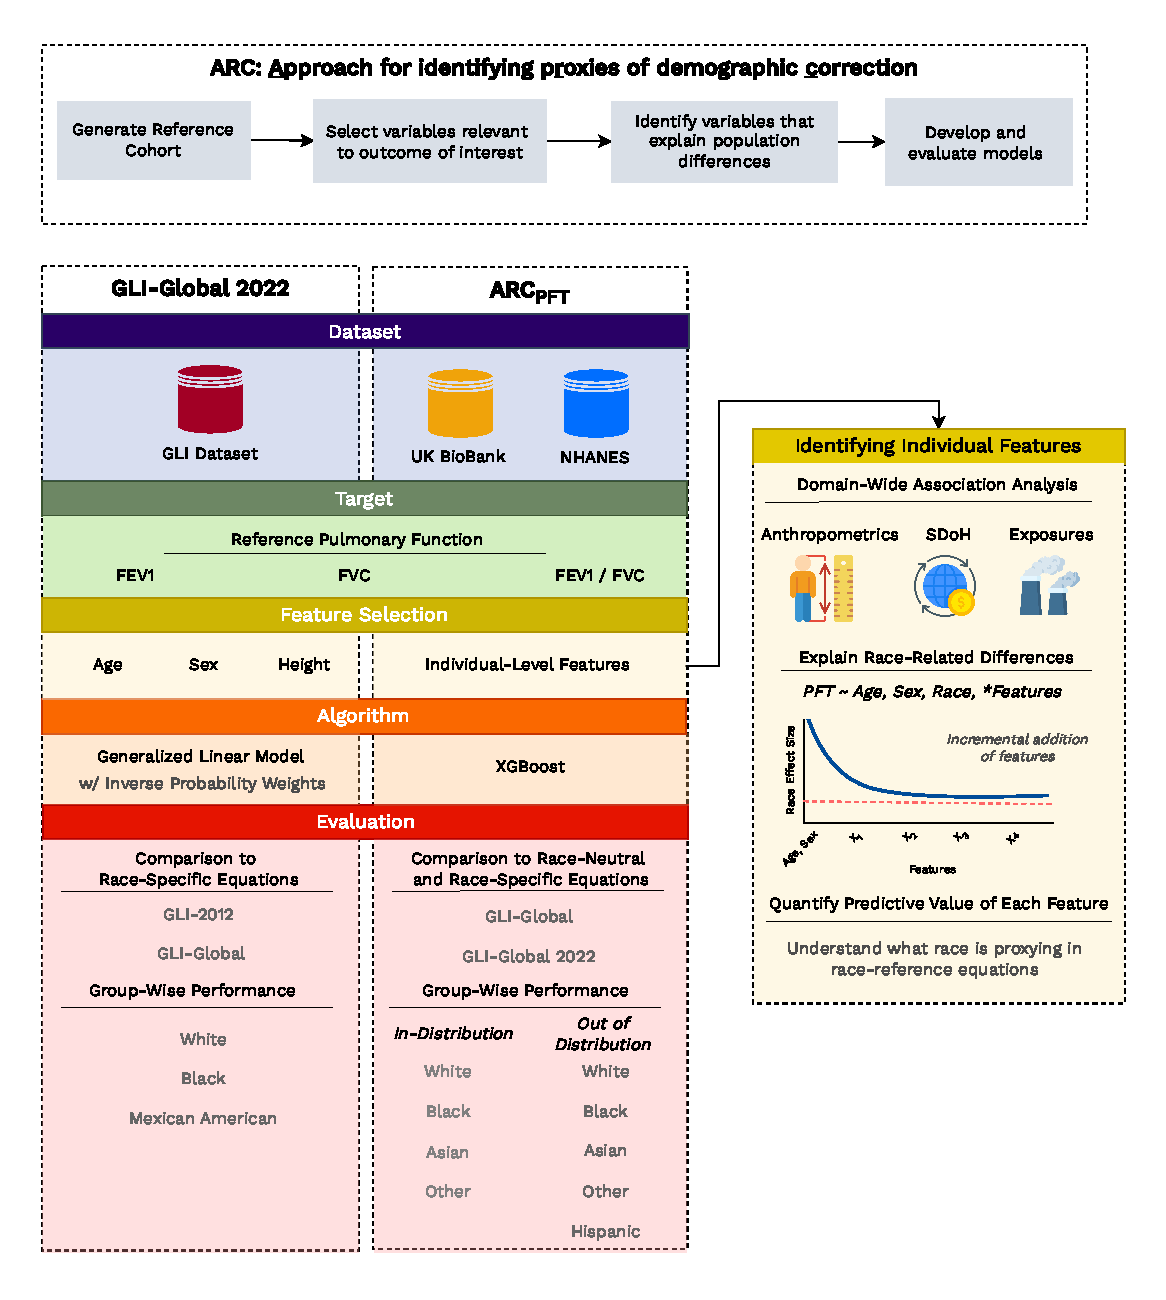
\includegraphics[width=\textwidth,height=0.78\textheight,keepaspectratio]{figures/schematic.pdf}
\caption{\textbf{Overview of the GLI-Global and ARC$_{\mathrm{PFT}}$ frameworks for removing the use of race in reference pulmonary function test equations.} The GLI-Global equation uses the GLI dataset to model reference pulmonary function (FEV$_1$, FVC) with generalized linear models using age, sex, and height as predictors. This equation is evaluated against race-adjusted equations (GLI-2012) and assessed for groupwise performance across White, Black, and Mexican American populations. The ARC$_{\mathrm{PFT}}$ equation uses UK Biobank and NHANES datasets, employing XGBoost models with individual-level features that explain race-related differences. The framework compares race-neutral (GLI-Global) and race-specific (GLI-2012) equations and evaluates groupwise performance both in-distribution and out-of-distribution across diverse race groups.}
\label{fig:schematic}
\vspace{2pt}
\end{figure}
\clearpage

\begin{figure}[H]
\centering
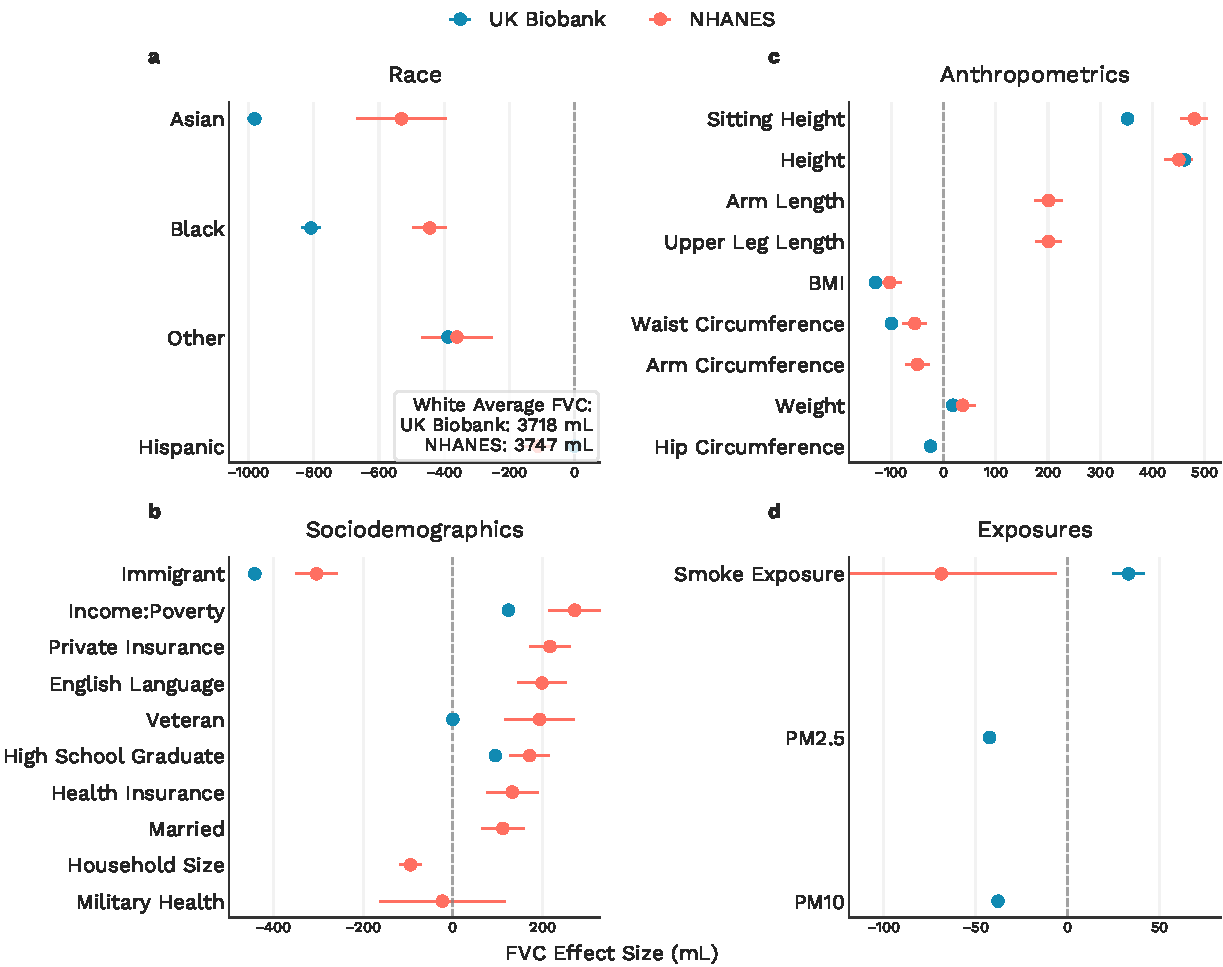
\includegraphics[width=\textwidth,height=0.78\textheight,keepaspectratio]{figures/ewas_fvc.pdf}
\caption{\textbf{Associations of Race, Sociodemographics, Anthropometrics, and Exposures with FVC (mL).} Effect sizes are cohort-specific linear regression coefficients from models adjusted for age, sex, and an age-by-sex interaction, with error bars showing $\pm$1 SE. Continuous predictors were standardized within cohort, so effect sizes correspond to a 1-SD increase. \textbf{(A)}~Race. White participants are the reference group, and the dashed line marks the null effect. Self-reported categories were harmonized across cohorts, with Asian and South Asian combined, and Hispanic shown only in NHANES. The annotation reports mean FVC among White participants in each cohort. \textbf{(B)}~Sociodemographics. Immigrant status indicates being born outside the study country, with native-born as the reference. The poverty indicator contrasts participants at or above the poverty threshold with those below it, using NHANES income-to-poverty ratio and UK Biobank income relative to the UK poverty threshold. Other binary variables compare the presence versus absence of the characteristic, and household size reflects the number of household members. \textbf{(C)}~Anthropometrics. Sitting height was available in UK Biobank and NHANES III and was imputed for NHANES IV to support consistent modeling across cohorts. \textbf{(D)}~Exposures. Smoke exposure reflects any reported exposure at home or work, with no exposure as the reference. PM2.5 and PM10 reflect particulate matter exposures and are modeled as standardized continuous variables.}
\label{fig:ewas_fvc}
\vspace{2pt}
\end{figure}
\clearpage

\begin{figure}[H]
\centering
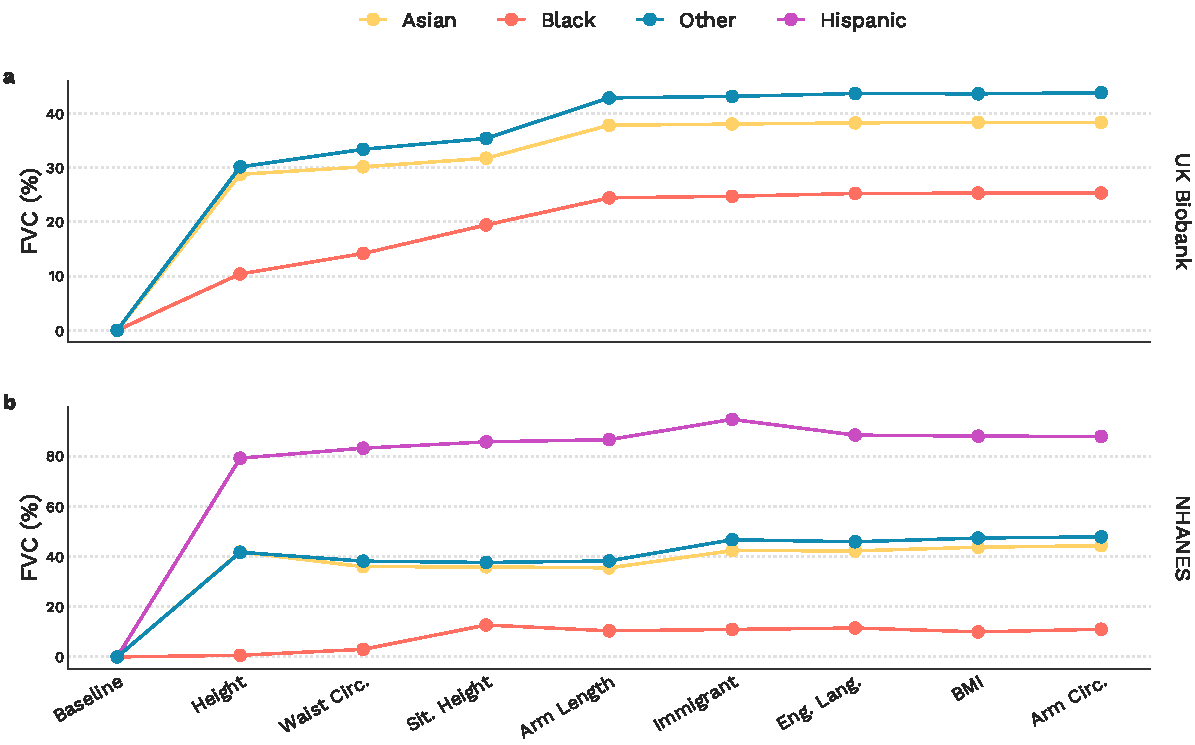
\includegraphics[width=\textwidth,height=0.78\textheight,keepaspectratio]{figures/explain_fvc_pct.pdf}
\caption{\textbf{Race-Related Differences Explained by Anthropometrics, Sociodemographics, and Exposure Variables on FVC in Healthy, Asymptomatic Individuals (\%).} For the \textbf{(A)}~UK Biobank and \textbf{(B)}~NHANES cohorts, the proportion of race-related differences in FVC (adjusted for age and sex) explained by stepwise inclusion of individual-level variables is shown. Cubic splines were applied to continuous variables to account for non-linear relationships.}
\label{fig:explain_fvc_pct}
\vspace{2pt}
\end{figure}
\clearpage

\begin{figure}[H]
\centering
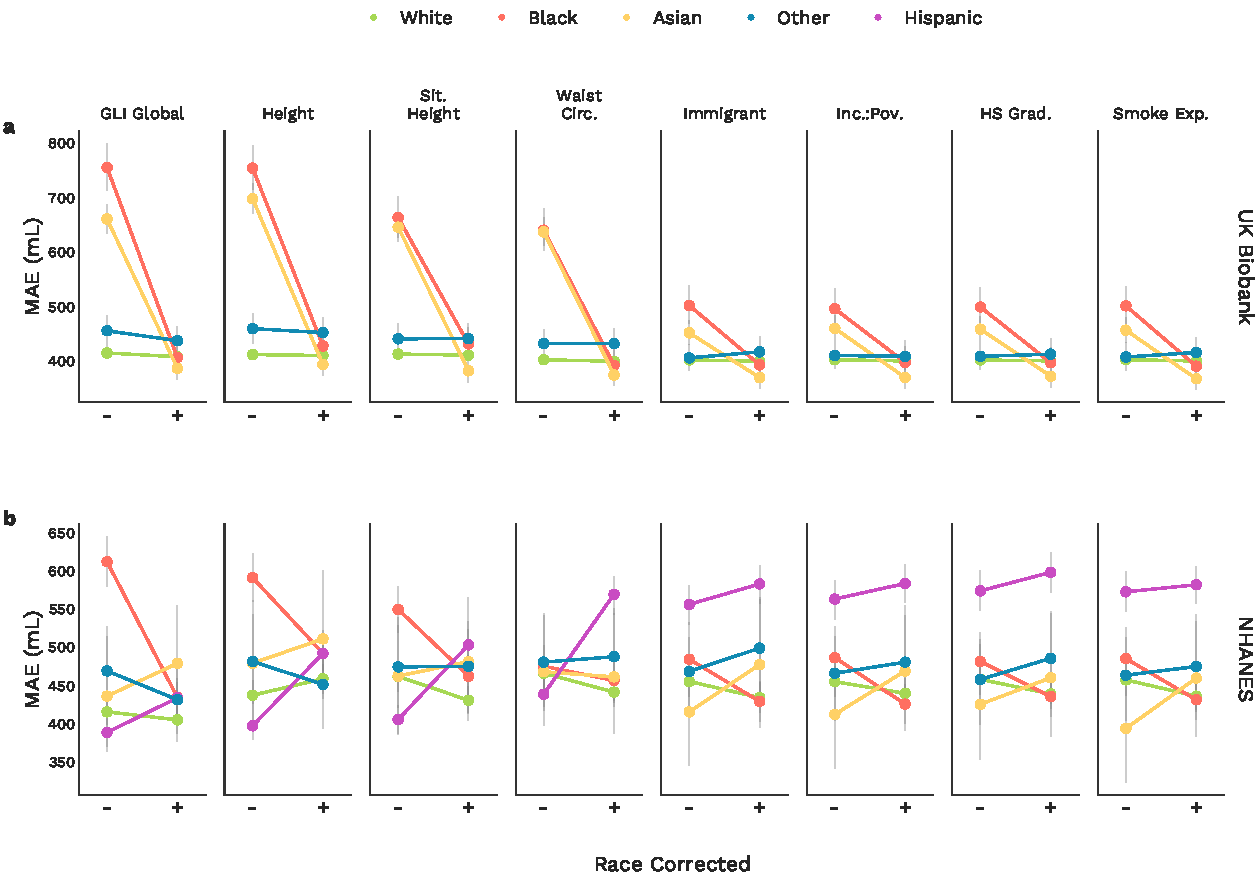
\includegraphics[width=\textwidth,height=0.78\textheight,keepaspectratio]{figures/train_fvc_ukb.pdf}
\caption{\textbf{Performance of GLI-Global and ARC\textsubscript{PFT} Models on Reference FVC Prediction.} Each model was trained on a subset of the UK Biobank ($n$ = 100,938) with age, sex, and height as baseline predictors. Sitting height, waist circumference, immigration status, and smoke exposure were incrementally added. MAE is shown for each race group with and without race adjustment. Hispanic was encoded as Other due to the absence of self-reported Hispanic individuals in UK Biobank. \textbf{(A)}~In-distribution evaluation on the UK Biobank held-out test set ($n$ = 43,260). \textbf{(B)}~Out-of-distribution evaluation on NHANES ($n$ = 3,354).}
\label{fig:train_fvc_ukb}
\vspace{2pt}
\end{figure}
\clearpage

\section*{Figures}
\setcounter{figure}{0}
\renewcommand{\figurename}{Supplementary Fig.}
\renewcommand{\thefigure}{\arabic{figure}}

\begin{figure}[H]
\centering
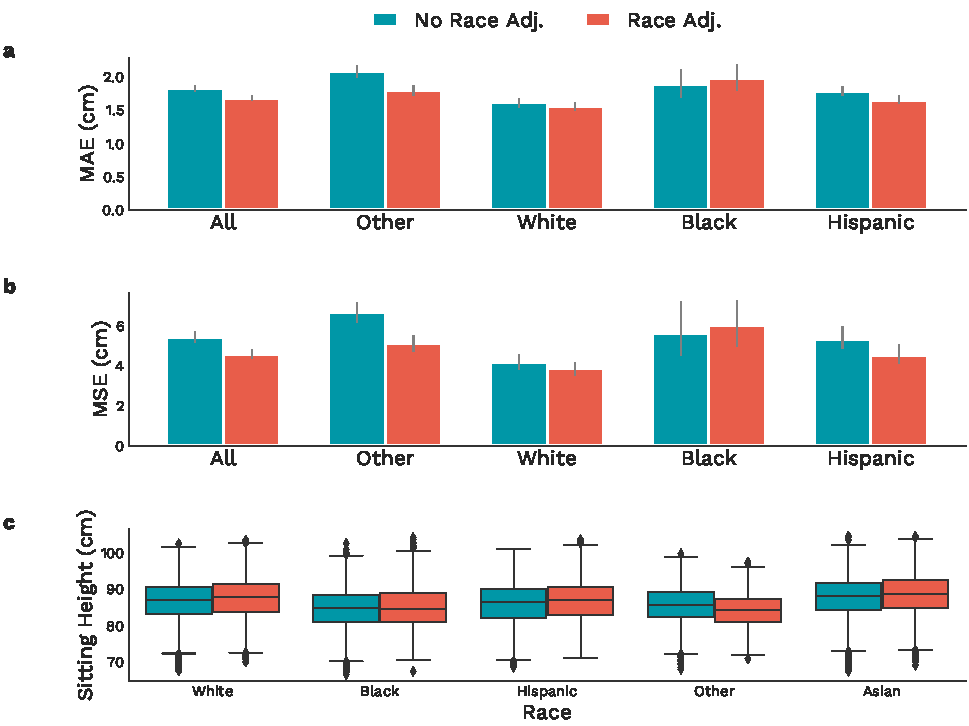
\includegraphics[width=\textwidth,height=0.78\textheight,keepaspectratio]{figures/imputation.pdf}
\caption{\textbf{Sitting Height Prediction Performance.} XGBoost models predicted sitting height (cm) from age, height, and upper-leg length, trained in NHANES III using an 80/20 split. Test error was reported overall and stratified by race. \textbf{(A)}~Mean absolute error (MAE; cm). \textbf{(B)}~Mean squared error (MSE). Bars show group means; error bars show 95\% bootstrap confidence intervals (1,000 resamples). Race adjustment improved prediction but was not used in the imputation model. \textbf{(C)}~NHANES IV distribution of imputed sitting height (cm) by race. Box plots show the median and interquartile range (IQR); whiskers extend to 1.5$\times$IQR; points denote outliers.}
\label{fig:imputation}
\vspace{2pt}
\end{figure}
\clearpage

\begin{figure}[H]
\centering
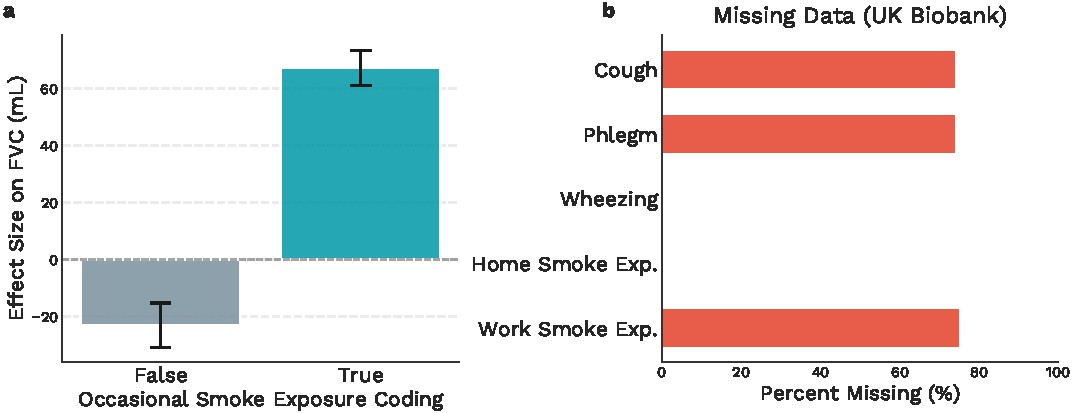
\includegraphics[width=\textwidth,height=0.78\textheight,keepaspectratio]{figures/data_quality.pdf}
\caption{\textbf{Data Quality in UK Biobank.} \textbf{(A)}~Effect of smoke exposure coding on FVC (mL). Smoke exposure was self-reported as never, don't know, occasionally, or often. Responses were encoded to a binary exposure variable: ``never'' and ``don't know'' were coded as unexposed, and ``often'' as exposed. Two alternative codings of ``occasionally'' are shown: Occasional = False codes ``occasionally'' as unexposed, whereas Occasional = True codes ``occasionally'' as exposed. This recoding reversed the estimated association with FVC: with Occasional = False, exposure was associated with lower FVC (negative effect), whereas with Occasional = True, exposure was associated with higher FVC (positive effect). Bars show estimated effect sizes on FVC (mL), and vertical lines indicate 95\% confidence intervals. \textbf{(B)}~Percentage of missing values for respiratory symptoms and exposures.}
\label{fig:data_quality}
\vspace{2pt}
\end{figure}
\clearpage

\begin{figure}[H]
\centering
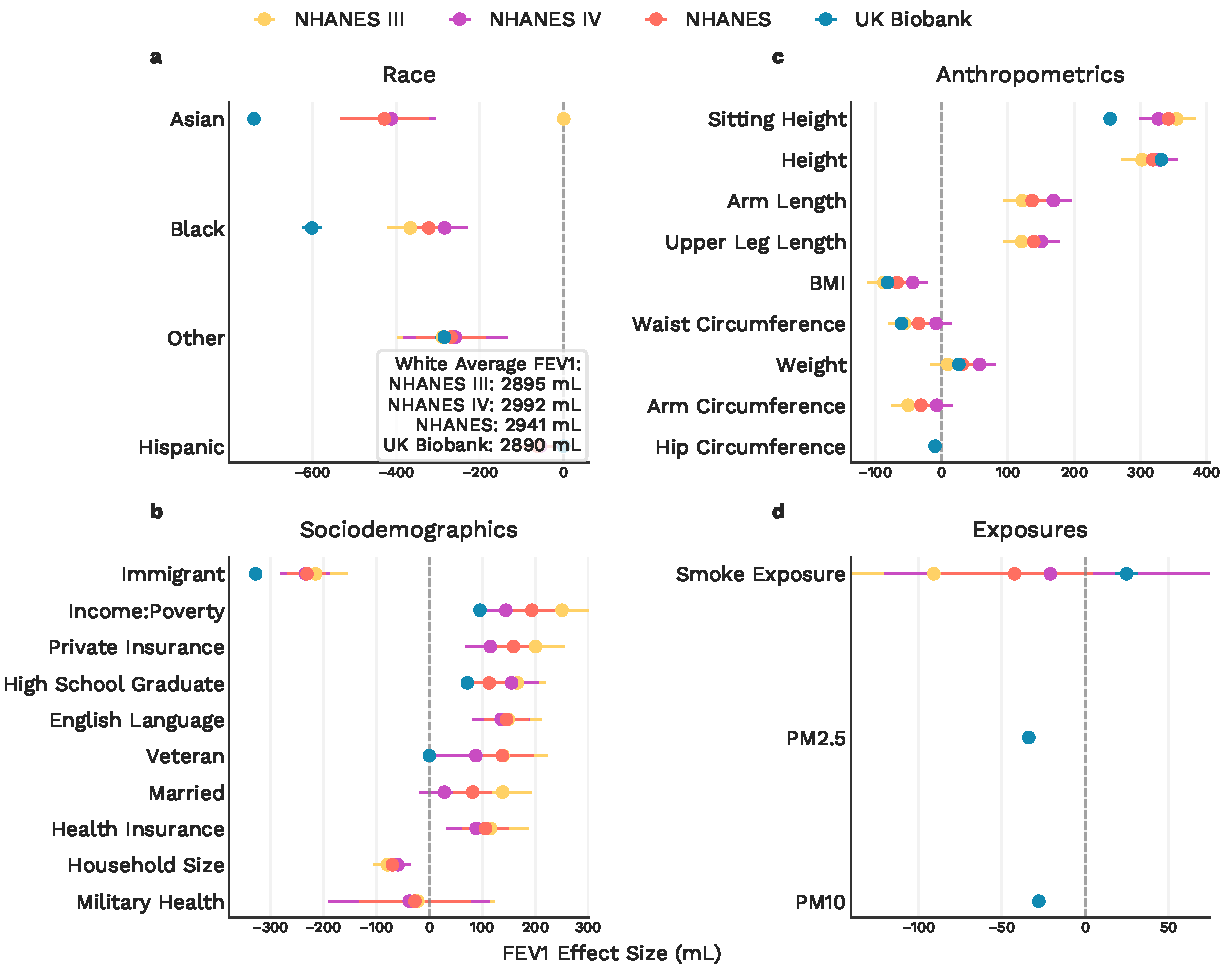
\includegraphics[width=\textwidth,height=0.78\textheight,keepaspectratio]{figures/ewas_fev1.pdf}
\caption{\textbf{Associations of Race, Sociodemographics, Anthropometrics, and Exposures with FEV$_1$ (mL).} Effect sizes are cohort-specific linear regression coefficients from models adjusted for age, sex, and an age-by-sex interaction, with error bars showing $\pm$1 SE. Continuous predictors were standardized within cohort, so effect sizes correspond to a 1-SD increase. \textbf{(A)}~Race. White participants are the reference group, and the dashed line marks the null effect. Self-reported categories were harmonized across cohorts, with Asian and South Asian combined, and Hispanic shown only in NHANES. The annotation reports mean FEV$_1$ among White participants in each cohort. \textbf{(B)}~Sociodemographics. Immigrant status indicates being born outside the study country, with native-born as the reference. The poverty indicator contrasts participants at or above the poverty threshold with those below it, using NHANES income-to-poverty ratio and UK Biobank income relative to the UK poverty threshold. Other binary variables compare the presence versus absence of the characteristic, and household size reflects the number of household members. \textbf{(C)}~Anthropometrics. Sitting height was available in UK Biobank and NHANES III and was imputed for NHANES IV to support consistent modeling across cohorts. \textbf{(D)}~Exposures. Smoke exposure reflects any reported exposure at home or work, with no exposure as the reference. PM2.5 and PM10 reflect particulate matter exposures and are modeled as standardized continuous variables.}
\label{fig:ewas_fev1}
\vspace{2pt}
\end{figure}
\clearpage

\begin{figure}[H]
\centering
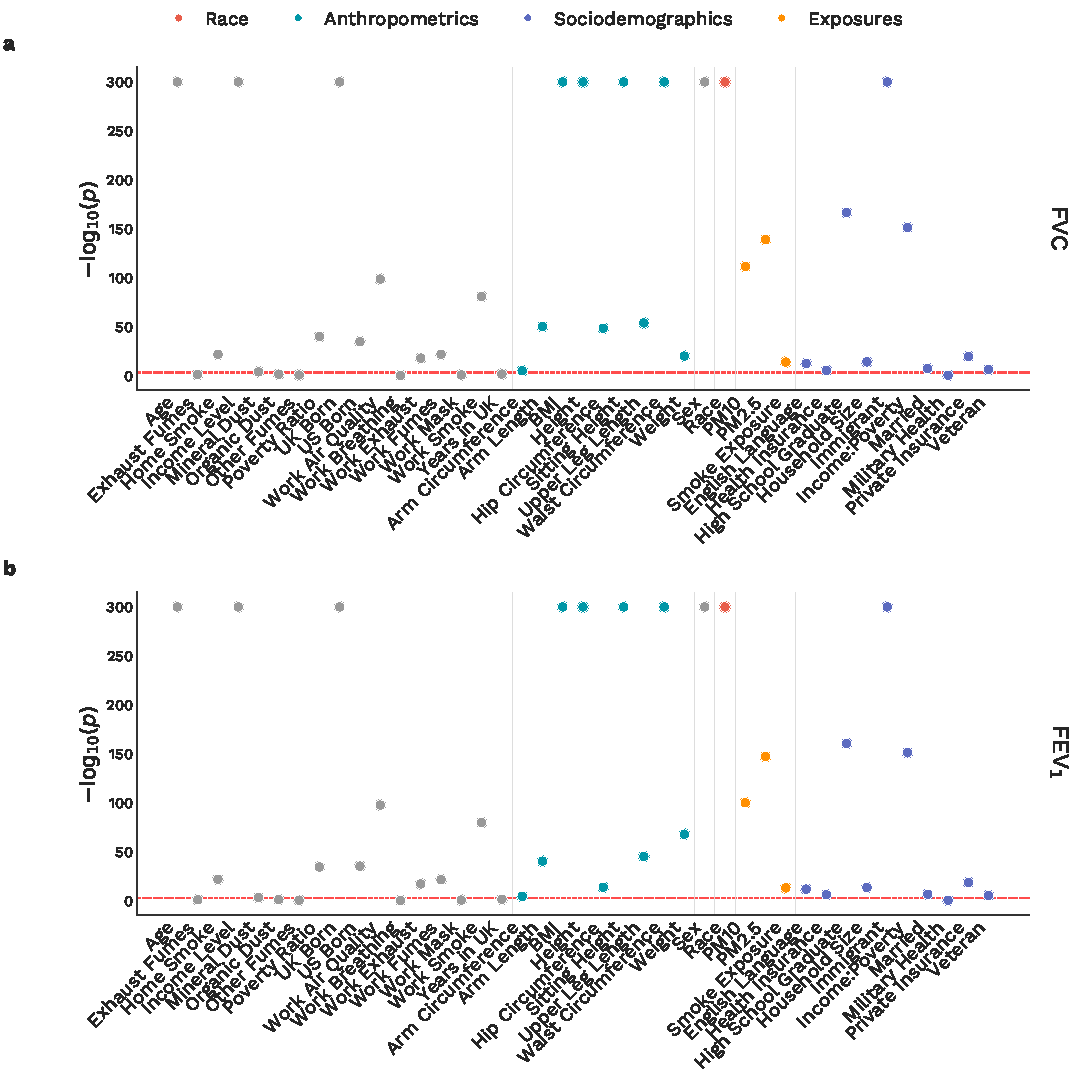
\includegraphics[width=\textwidth,height=0.78\textheight,keepaspectratio]{figures/manhattan.pdf}
\caption{\textbf{Significance of Variable Associations with Pulmonary Function Tests.} Each point represents a single variable association, plotted as $-\log_{10}(p)$ and colored by category (race, sociodemographics, anthropometrics, or exposures). The dashed red line marks the Bonferroni-corrected significance threshold ($\alpha = 0.05 / k$; $k = 38$ for UK Biobank, $k = 48$ for NHANES). \textbf{(A)}~FVC. \textbf{(B)}~FEV$_1$.}
\label{fig:manhattan}
\vspace{2pt}
\end{figure}
\clearpage

\begin{figure}[H]
\centering
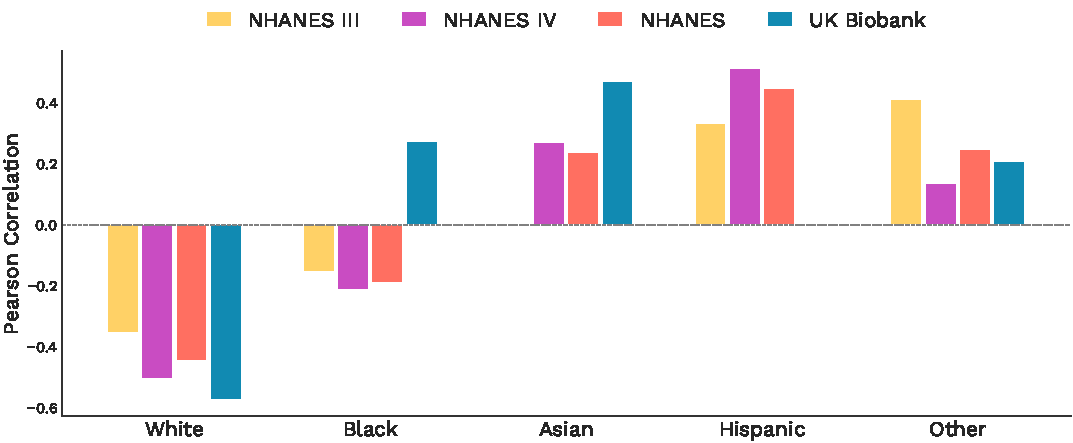
\includegraphics[width=\textwidth,height=0.78\textheight,keepaspectratio]{figures/immigrant_race_corr.pdf}
\caption{\textbf{Correlation of Immigrant Status with Race/Ethnicity Across Cohorts.} Pearson correlation coefficients between immigrant status and race/ethnicity indicators are shown for UK Biobank and NHANES (III, IV, and combined III--IV). The dashed line marks zero correlation. Asterisks indicate Bonferroni-adjusted $p < 0.05$ within cohort.}
\label{fig:immigrant_race_corr}
\vspace{2pt}
\end{figure}
\clearpage

\begin{figure}[H]
\centering
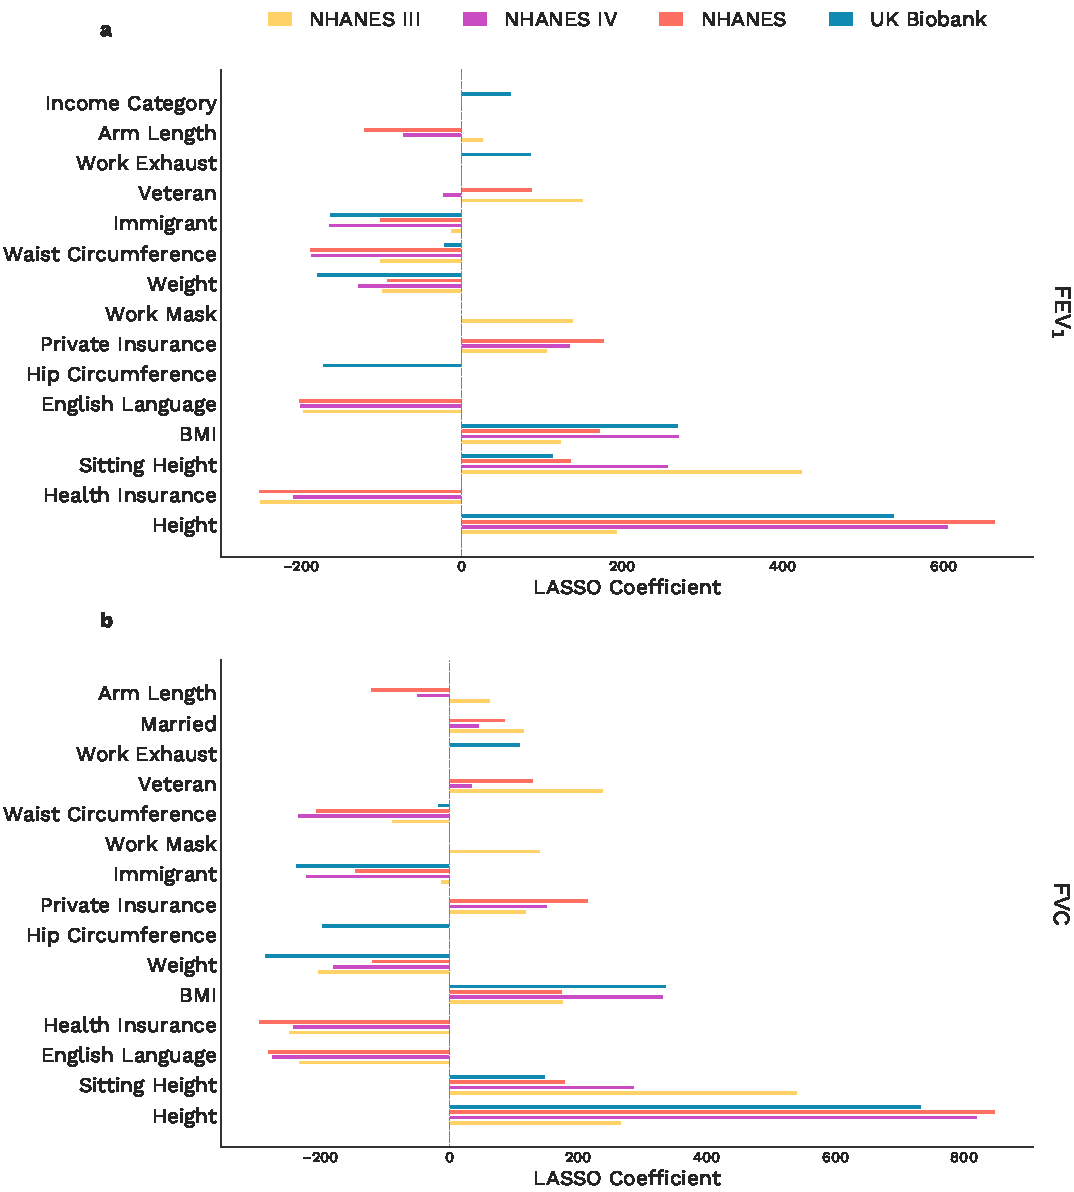
\includegraphics[width=\textwidth,height=0.78\textheight,keepaspectratio]{figures/lasso.pdf}
\caption{\textbf{Proxy Effect Sizes in Regularized Prediction Models Across Cohorts.} Fitted coefficients from lasso regression models predicting spirometry outcomes using an expanded feature set that includes all main effects and pairwise interactions among proxy variables. Models were fit separately in each cohort (UK Biobank, NHANES III--IV combined, NHANES III only, NHANES IV only) using 10-fold cross-validation to select the regularization strength ($\lambda$) that minimized mean squared error. Only non-zero coefficients are displayed. \textbf{(A)}~FEV$_1$. \textbf{(B)}~FVC.}
\label{fig:lasso}
\vspace{2pt}
\end{figure}
\clearpage

\begin{figure}[H]
\centering
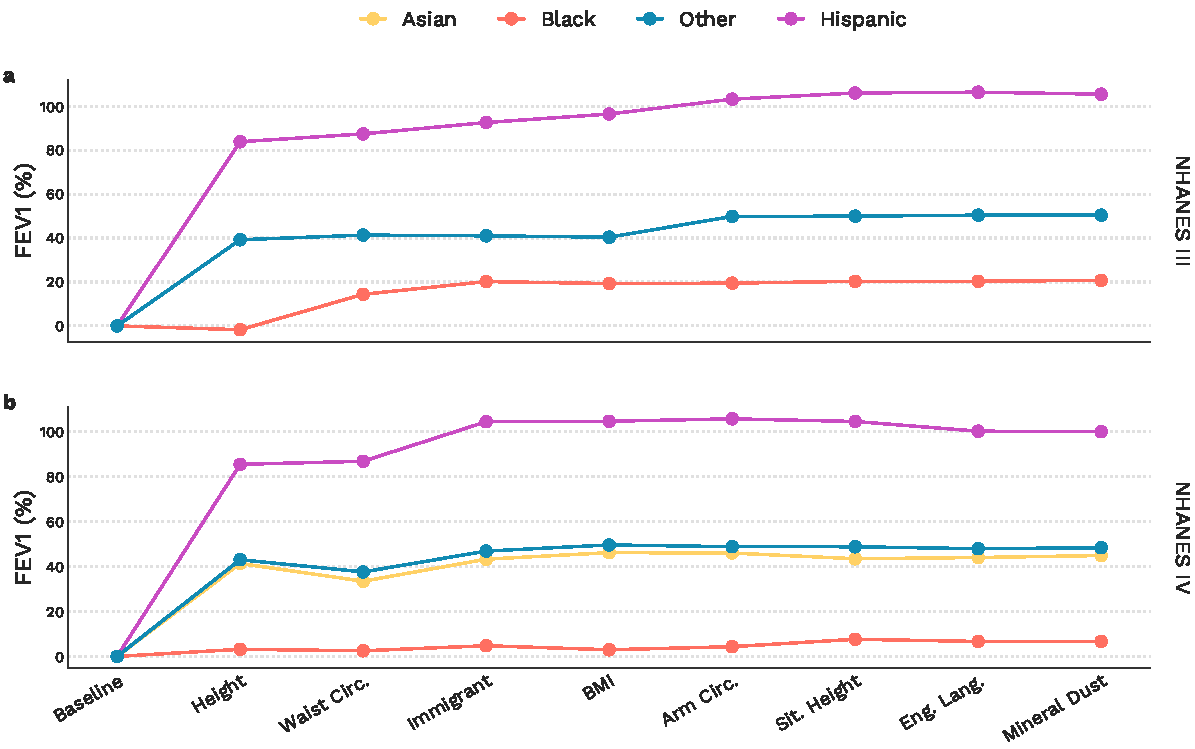
\includegraphics[width=\textwidth,height=0.78\textheight,keepaspectratio]{figures/explain_fev1_pct.pdf}
\caption{\textbf{Race-Related Differences Explained by Anthropometrics, Sociodemographics, and Exposure Variables on FEV$_1$ in Healthy, Asymptomatic Individuals (\%).} For the \textbf{(A)}~NHANES III and \textbf{(B)}~NHANES IV cohorts, the proportion of race-related differences in FEV$_1$ (adjusted for age and sex) explained by stepwise inclusion of individual-level variables is shown. Cubic splines were applied to continuous variables to account for non-linear relationships.}
\label{fig:explain_fev1_pct}
\vspace{2pt}
\end{figure}
\clearpage

\begin{figure}[H]
\centering
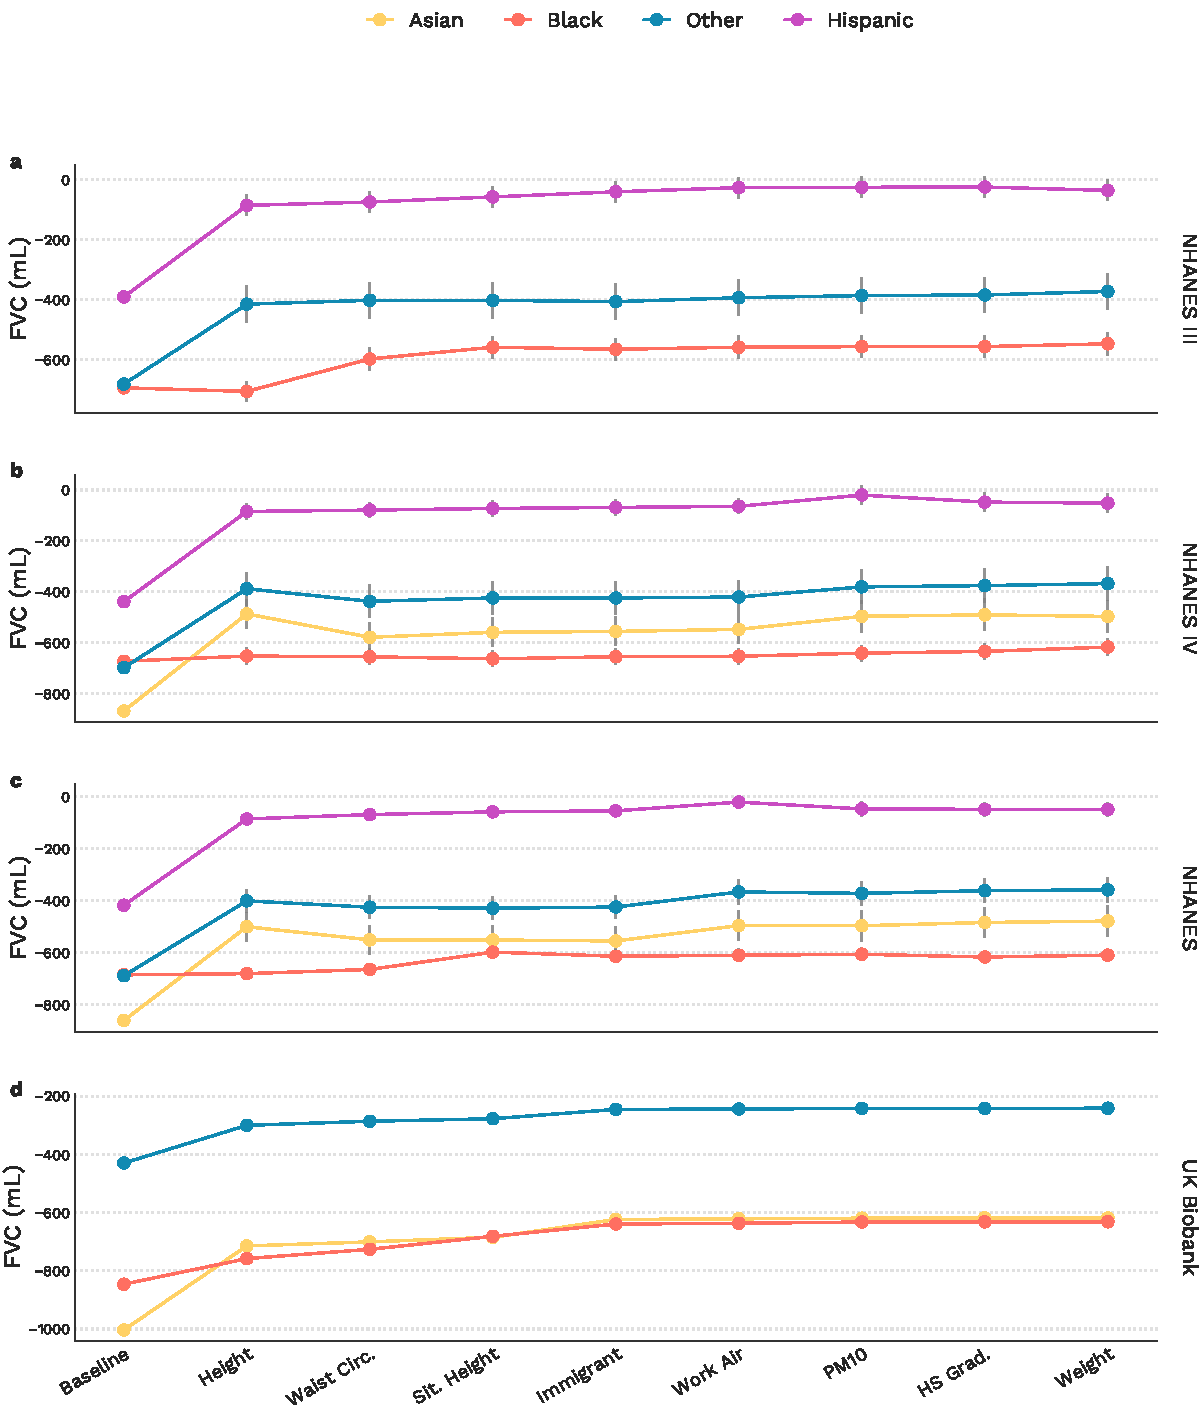
\includegraphics[width=\textwidth,height=0.78\textheight,keepaspectratio]{figures/explain_fvc_mL.pdf}
\caption{\textbf{Race-Related Differences Explained by Anthropometrics, Sociodemographics, and Exposure Variables on FVC in Healthy, Asymptomatic Individuals (mL).} For the \textbf{(A)}~NHANES III, \textbf{(B)}~NHANES IV, \textbf{(C)}~NHANES (III and IV combined), and \textbf{(D)}~UK Biobank cohorts, the proportion of race-related differences in FVC (adjusted for age and sex) explained by stepwise inclusion of individual-level variables is shown. Cubic splines were applied to continuous variables to account for non-linear relationships.}
\label{fig:explain_fvc_mL}
\vspace{2pt}
\end{figure}
\clearpage

\begin{figure}[H]
\centering
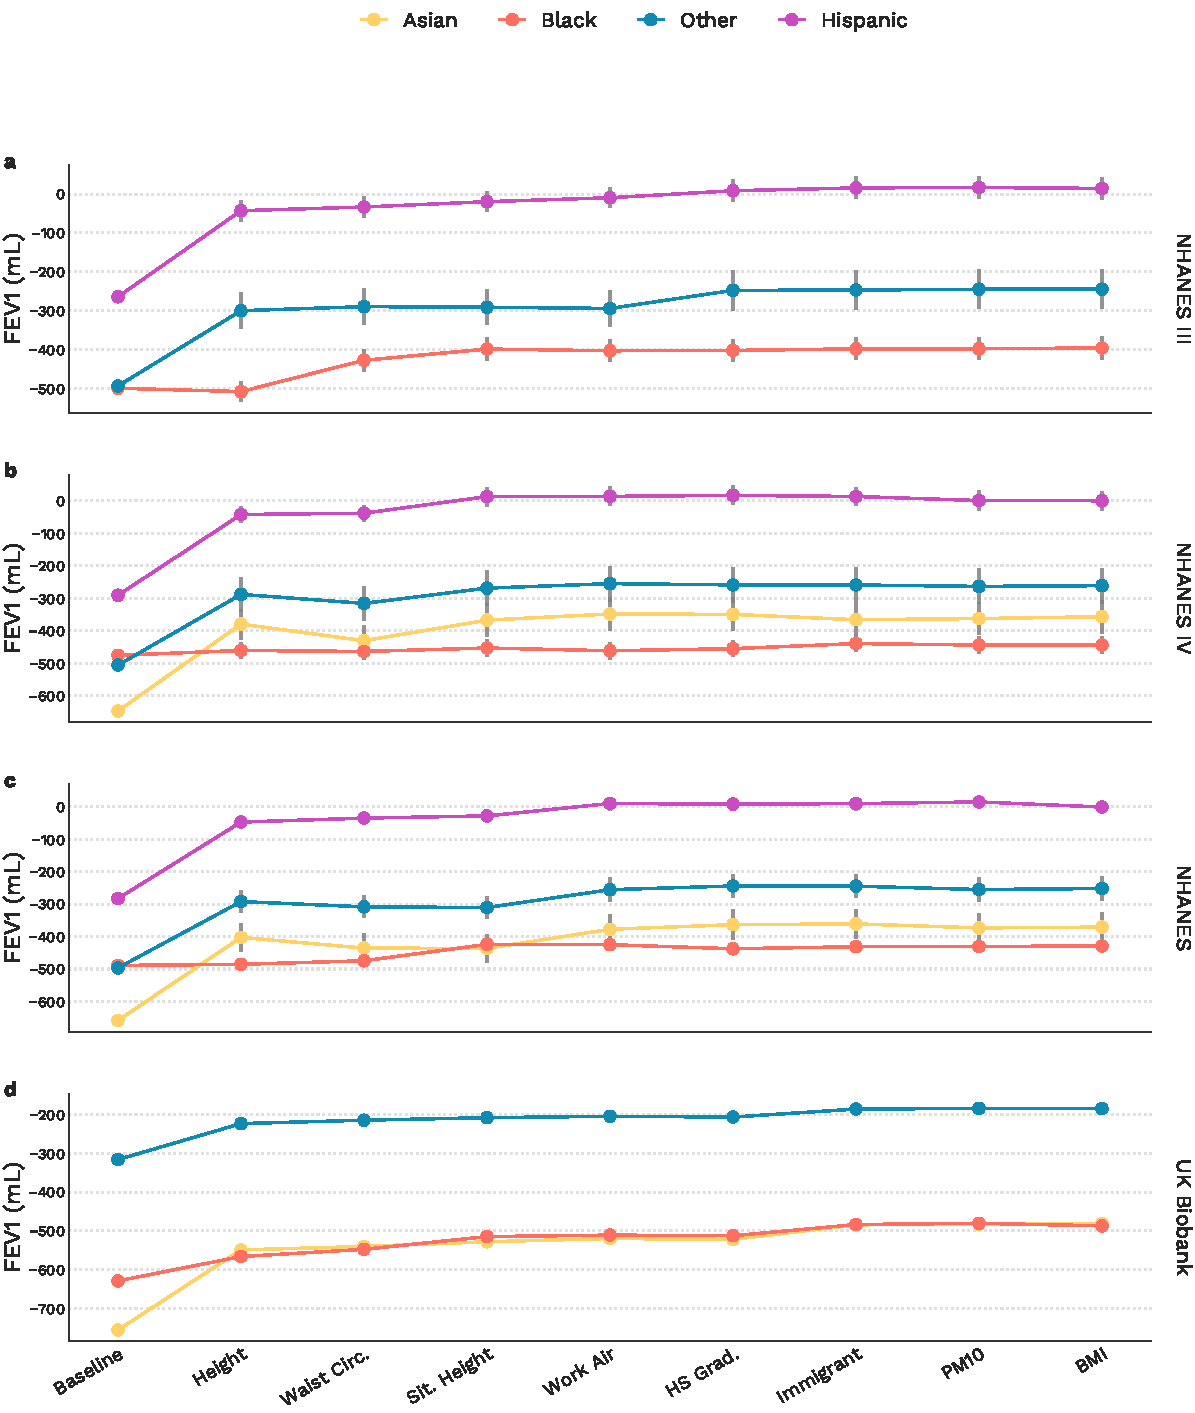
\includegraphics[width=\textwidth,height=0.78\textheight,keepaspectratio]{figures/explain_fev1_mL.pdf}
\caption{\textbf{Race-Related Differences Explained by Anthropometrics, Sociodemographics, and Exposure Variables on FEV$_1$ in Healthy, Asymptomatic Individuals (mL).} For the \textbf{(A)}~NHANES III, \textbf{(B)}~NHANES IV, \textbf{(C)}~NHANES (III and IV combined), and \textbf{(D)}~UK Biobank cohorts, the proportion of race-related differences in FEV$_1$ (adjusted for age and sex) explained by stepwise inclusion of individual-level variables is shown. Cubic splines were applied to continuous variables to account for non-linear relationships.}
\label{fig:explain_fev1_mL}
\vspace{2pt}
\end{figure}
\clearpage

\begin{figure}[H]
\centering
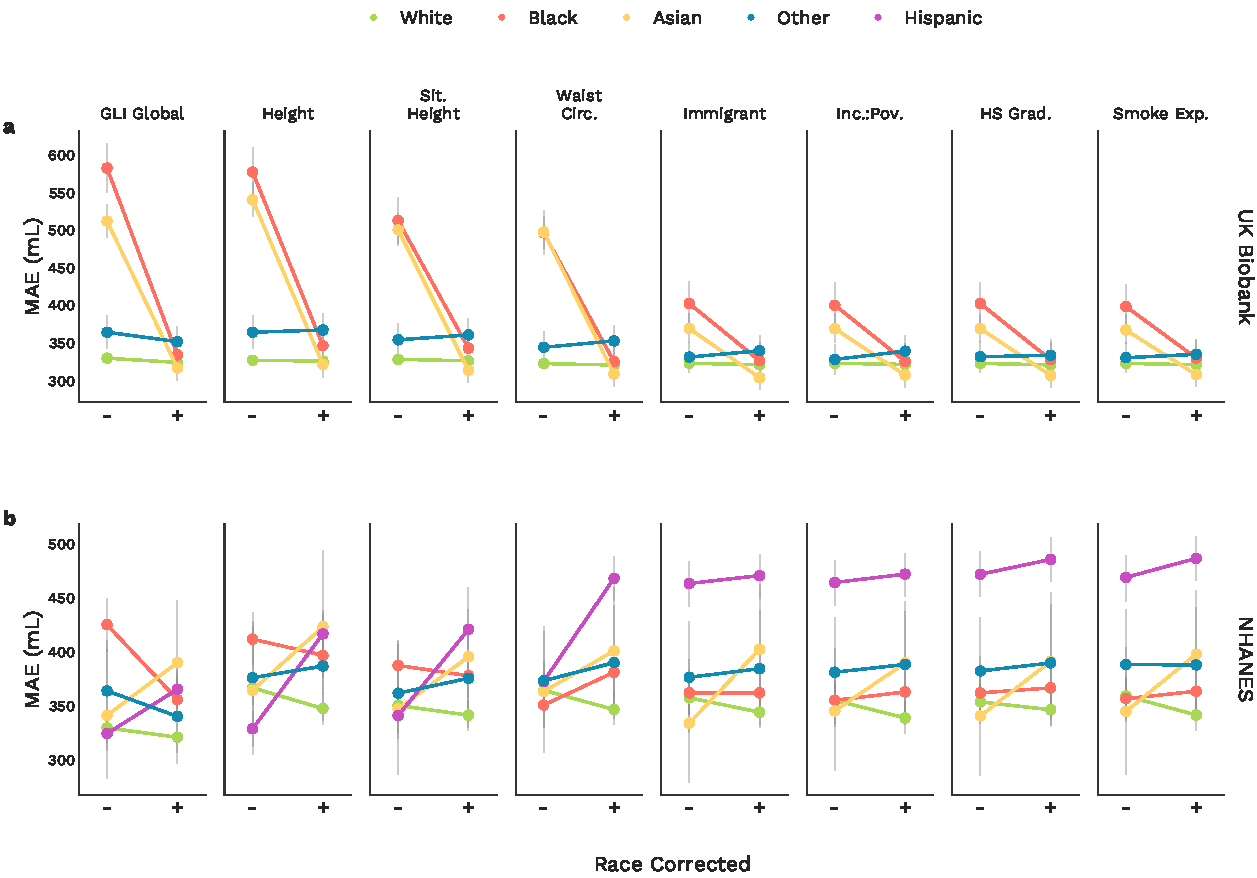
\includegraphics[width=\textwidth,height=0.78\textheight,keepaspectratio]{figures/train_fev1_ukb.pdf}
\caption{\textbf{Performance of GLI-Global and ARC\textsubscript{PFT} Models on Reference FEV$_1$ Prediction (Trained on UK Biobank).} Each model was trained on a subset of the UK Biobank with age, sex, and height as baseline predictors. Sitting height, waist circumference, immigration status, and smoke exposure were incrementally added. MAE is shown for each race group with and without race adjustment. Hispanic was encoded as Other due to the absence of labeled Hispanic individuals in UK Biobank. \textbf{(A)}~In-distribution evaluation on the UK Biobank held-out test set. \textbf{(B)}~Out-of-distribution evaluation on NHANES.}
\label{fig:train_fev1_ukb}
\vspace{2pt}
\end{figure}
\clearpage

\begin{figure}[H]
\centering
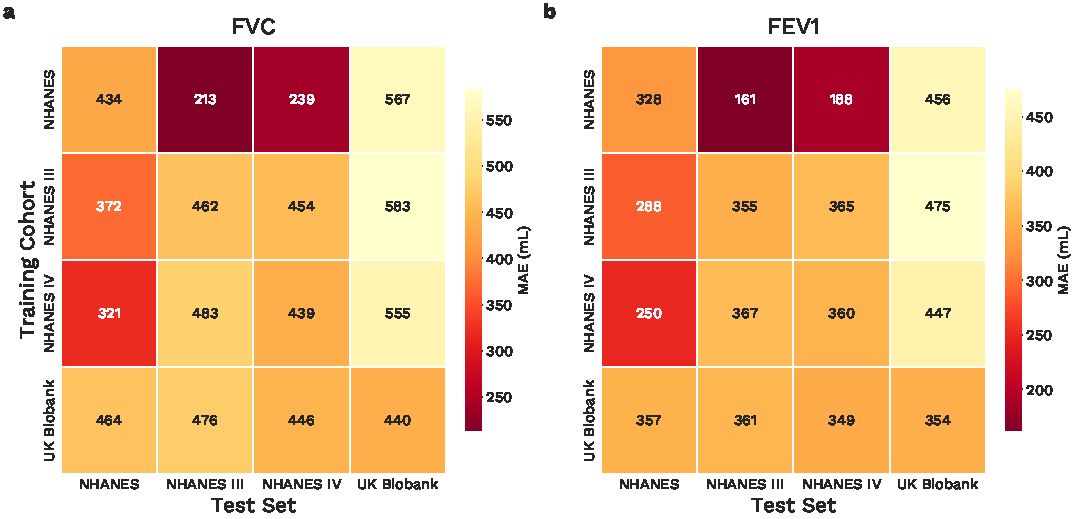
\includegraphics[width=\textwidth,height=0.78\textheight,keepaspectratio]{figures/train_heatmap.pdf}
\caption{\textbf{Cross-Cohort Prediction Mean Absolute Error Summary.} Each cell shows the mean absolute error (MAE), averaged across race groups, for the best-performing covariate configuration (without race adjustment). \textbf{(A)}~FVC. \textbf{(B)}~FEV$_1$.}
\label{fig:train_heatmap}
\vspace{2pt}
\end{figure}
\clearpage

\begin{figure}[H]
\centering
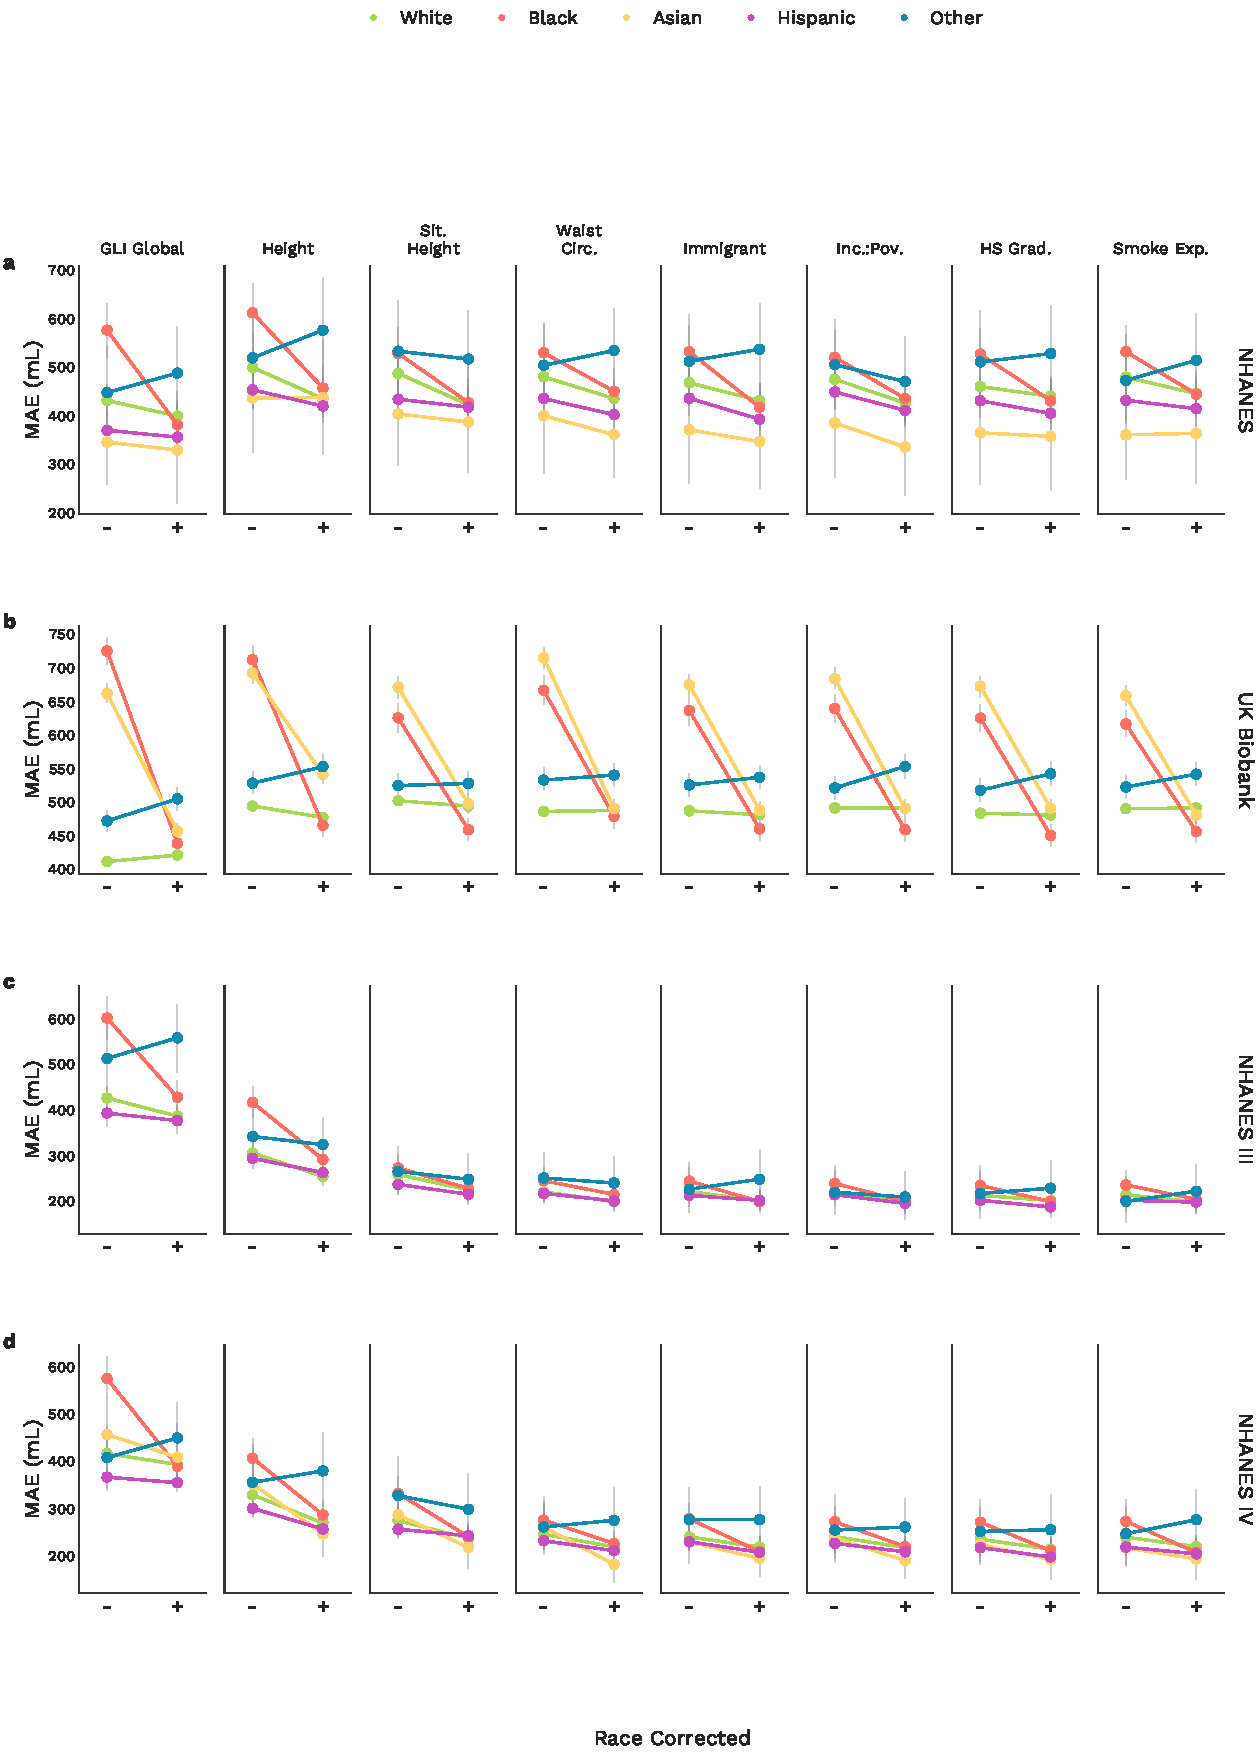
\includegraphics[width=\textwidth,height=0.78\textheight,keepaspectratio]{figures/train_fvc_nh.pdf}
\caption{\textbf{Performance of GLI-Global and ARC\textsubscript{PFT} Models on Reference FVC Prediction.} Models were trained on NHANES III and IV combined ($n$ = 2,347) with age, sex, and height as baseline predictors; sitting height, waist circumference, immigration status, and smoke exposure were incrementally added. MAE is shown for each race group with and without race adjustment. \textbf{(A)}~In-distribution evaluation on the NHANES held-out test set ($n$ = 1,007). \textbf{(B)}~Out-of-distribution evaluation on UK Biobank ($n$ = 144,198). \textbf{(C)}~Out-of-distribution evaluation on NHANES III ($n$ = 1,569). \textbf{(D)}~Out-of-distribution evaluation on NHANES IV ($n$ = 1,785).}
\label{fig:train_fvc_nh}
\vspace{2pt}
\end{figure}
\clearpage

\begin{figure}[H]
\centering
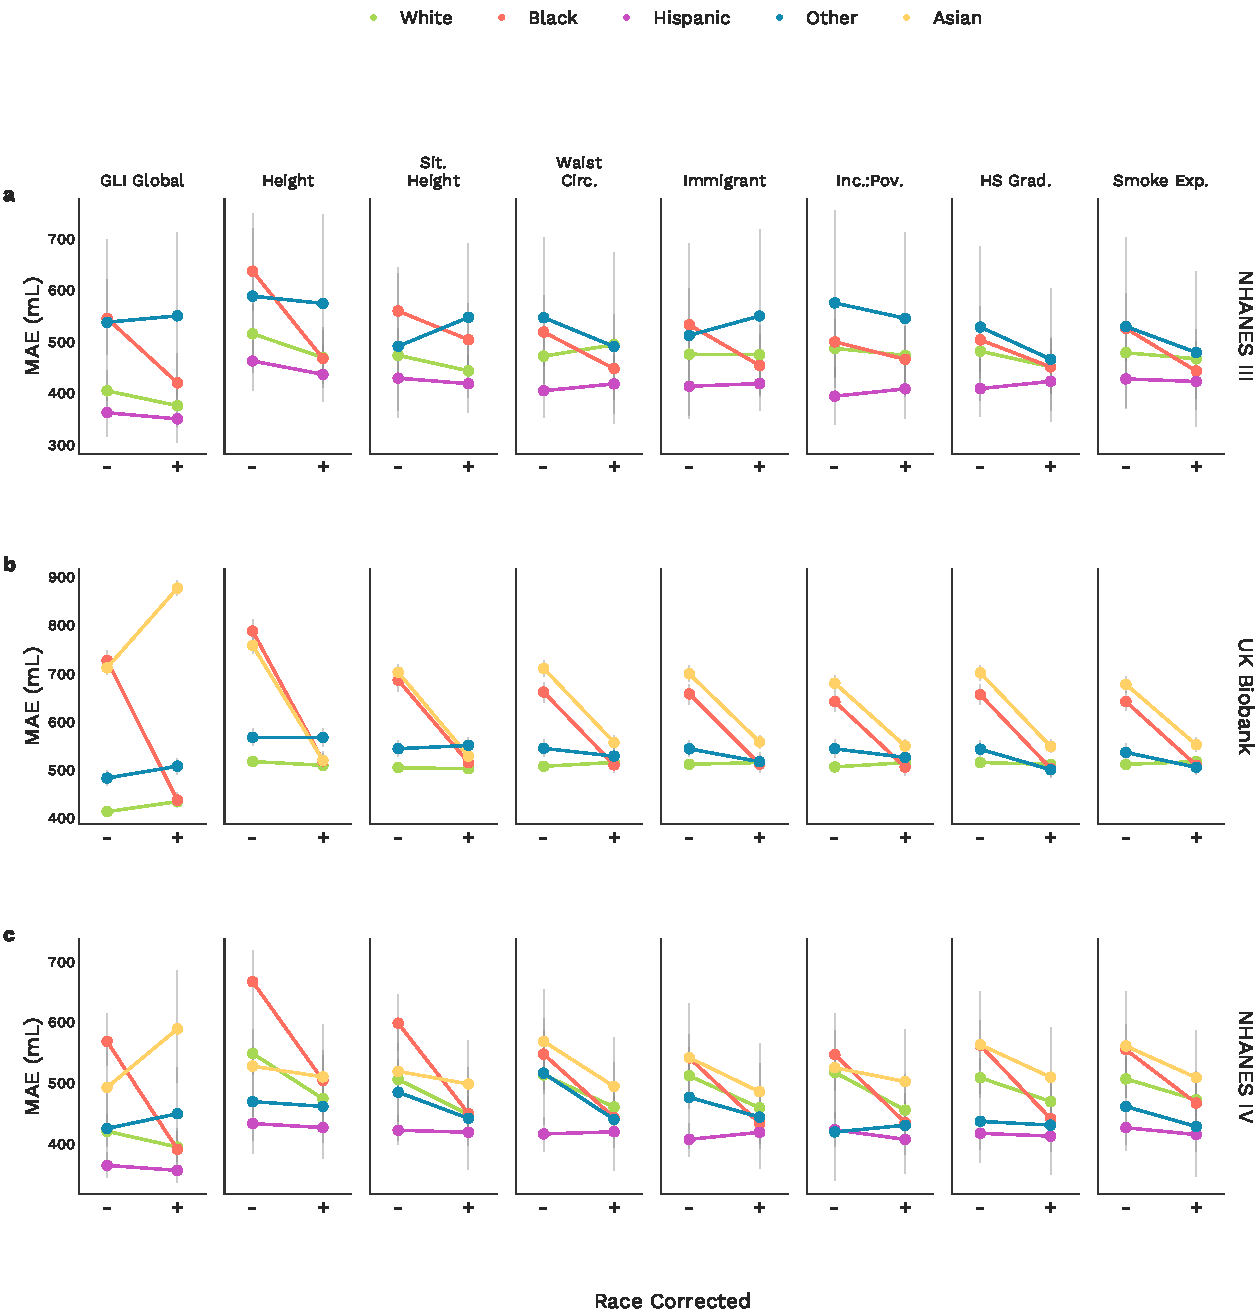
\includegraphics[width=\textwidth,height=0.78\textheight,keepaspectratio]{figures/train_fvc_nh3.pdf}
\caption{\textbf{Performance of GLI-Global and ARC\textsubscript{PFT} Models on Reference FVC Prediction.} Models were trained on NHANES III ($n$ = 1,098) with age, sex, and height as baseline predictors; sitting height, waist circumference, immigration status, and smoke exposure were incrementally added. MAE is shown for each race group with and without race adjustment. \textbf{(A)}~In-distribution evaluation on the NHANES III held-out test set ($n$ = 471). \textbf{(B)}~Out-of-distribution evaluation on UK Biobank ($n$ = 144,198). \textbf{(C)}~Out-of-distribution evaluation on NHANES IV ($n$ = 1,785).}
\label{fig:train_fvc_nh3}
\vspace{2pt}
\end{figure}
\clearpage

\begin{figure}[H]
\centering
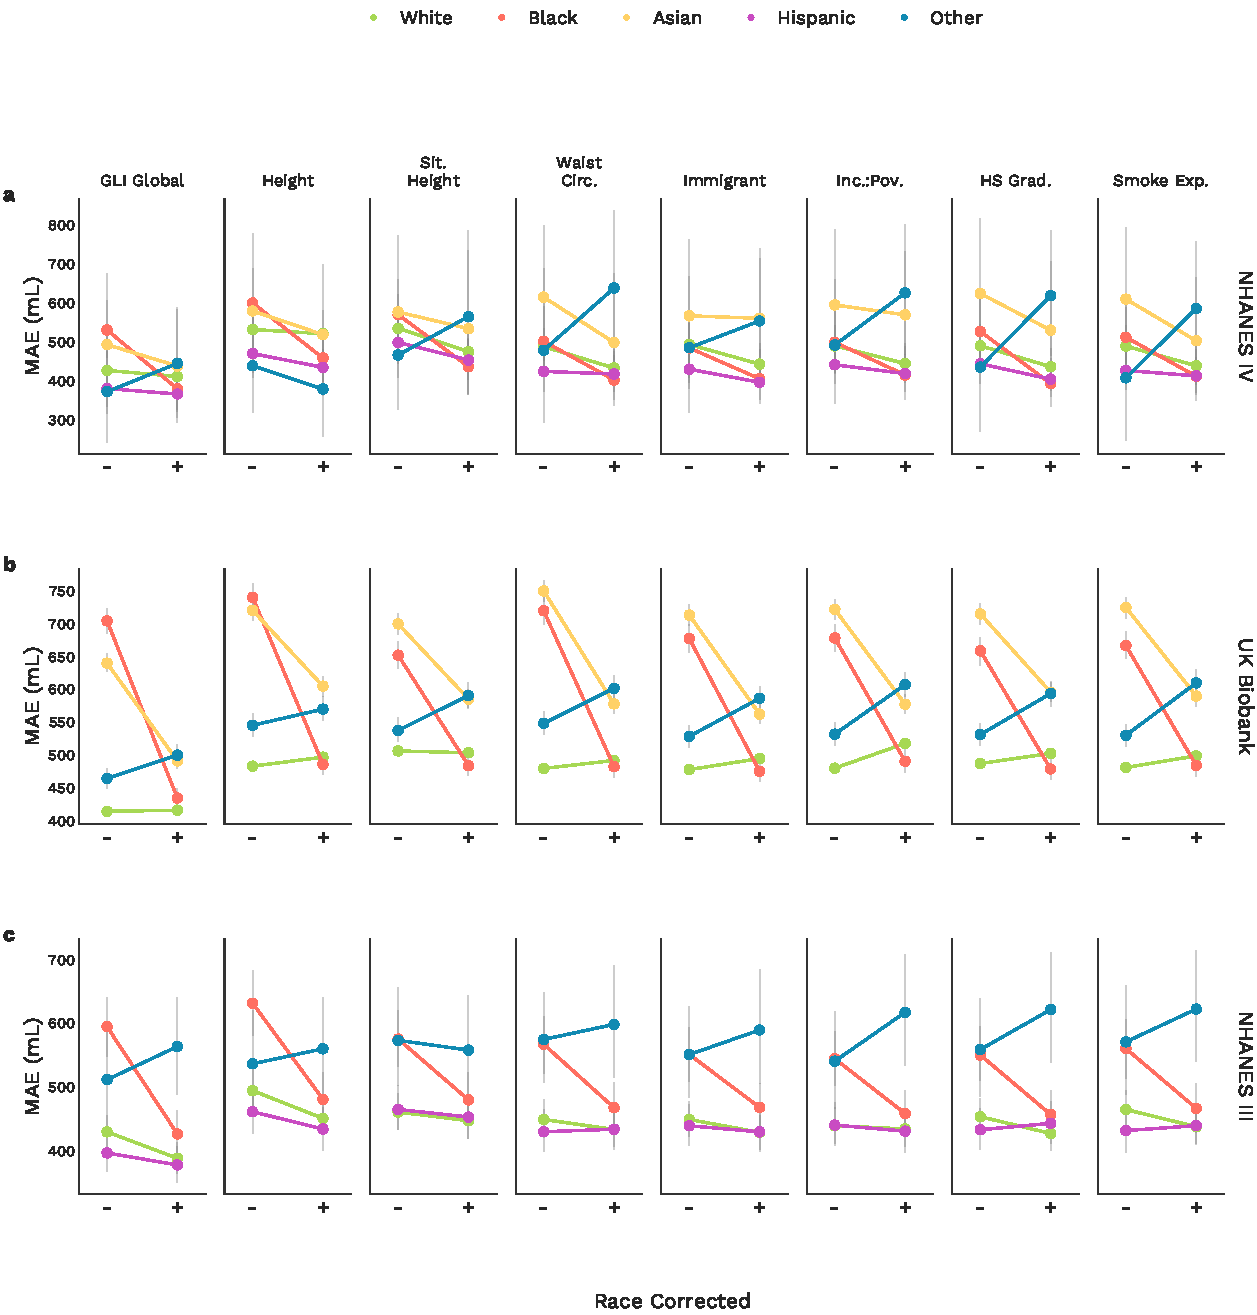
\includegraphics[width=\textwidth,height=0.78\textheight,keepaspectratio]{figures/train_fvc_nh4.pdf}
\caption{\textbf{Performance of GLI-Global and ARC\textsubscript{PFT} Models on Reference FVC Prediction.} Models were trained on NHANES IV ($n$ = 1,249) with age, sex, and height as baseline predictors; sitting height, waist circumference, immigration status, and smoke exposure were incrementally added. MAE is shown for each race group with and without race adjustment. \textbf{(A)}~In-distribution evaluation on the NHANES IV held-out test set ($n$ = 536). \textbf{(B)}~Out-of-distribution evaluation on UK Biobank ($n$ = 144,198). \textbf{(C)}~Out-of-distribution evaluation on NHANES III ($n$ = 1,569).}
\label{fig:train_fvc_nh4}
\vspace{2pt}
\end{figure}
\clearpage

\begin{figure}[H]
\centering
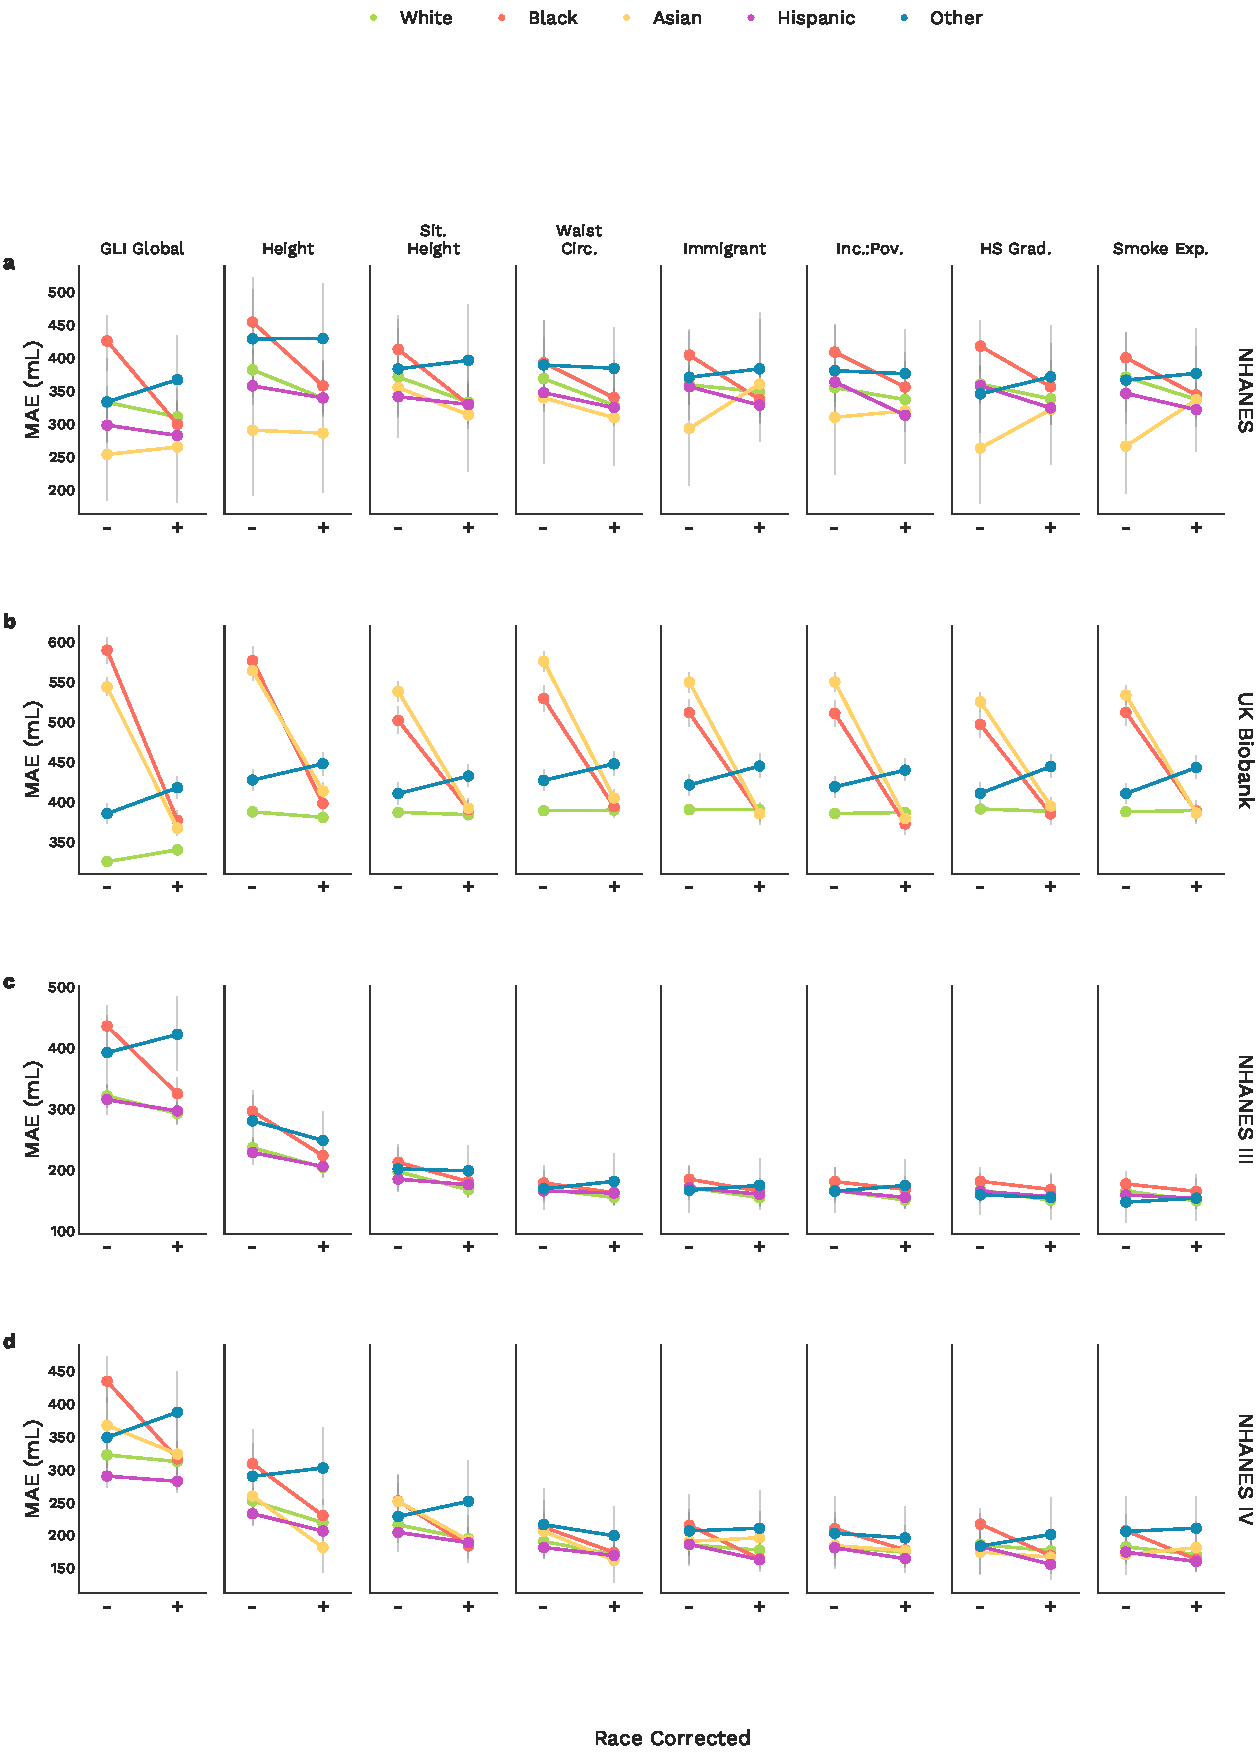
\includegraphics[width=\textwidth,height=0.78\textheight,keepaspectratio]{figures/train_fev1_nh.pdf}
\caption{\textbf{Performance of GLI-Global and ARC\textsubscript{PFT} Models on Reference FEV$_1$ Prediction.} Models were trained on NHANES III and IV combined ($n$ = 2,347) with age, sex, and height as baseline predictors; sitting height, waist circumference, immigration status, and smoke exposure were incrementally added. MAE is shown for each race group with and without race adjustment. \textbf{(A)}~In-distribution evaluation on the NHANES held-out test set ($n$ = 1,007). \textbf{(B)}~Out-of-distribution evaluation on UK Biobank ($n$ = 144,198). \textbf{(C)}~Out-of-distribution evaluation on NHANES III ($n$ = 1,569). \textbf{(D)}~Out-of-distribution evaluation on NHANES IV ($n$ = 1,785).}
\label{fig:train_fev1_nh}
\vspace{2pt}
\end{figure}
\clearpage

\begin{figure}[H]
\centering
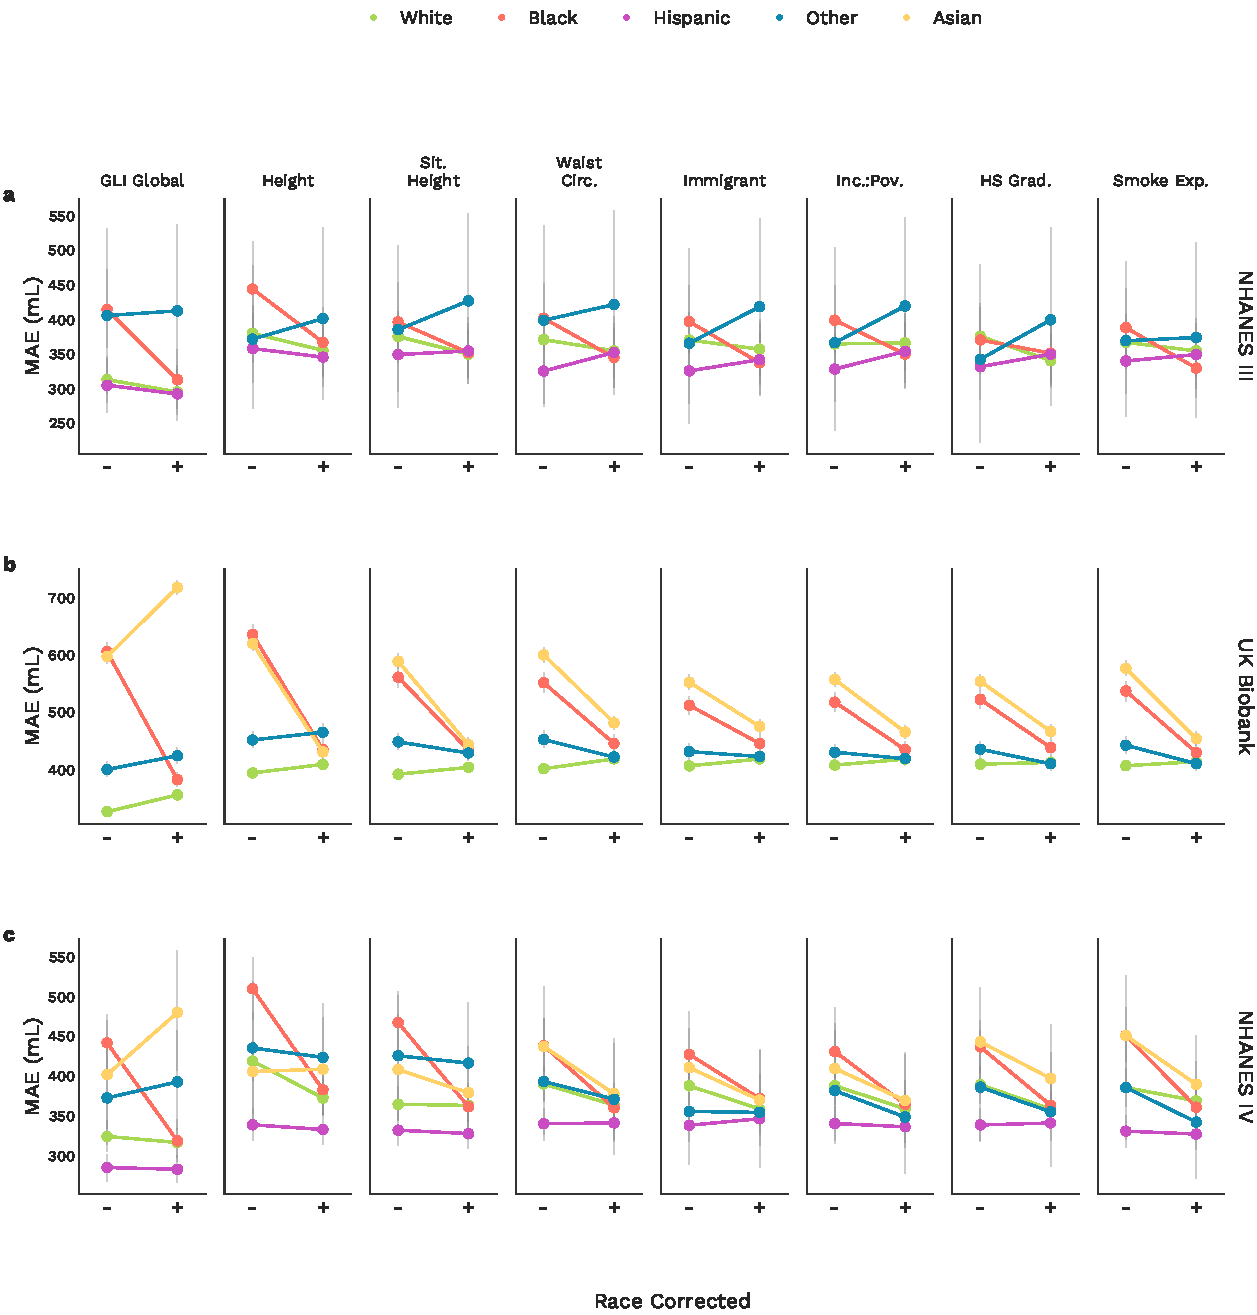
\includegraphics[width=\textwidth,height=0.78\textheight,keepaspectratio]{figures/train_fev1_nh3.pdf}
\caption{\textbf{Performance of GLI-Global and ARC\textsubscript{PFT} Models on Reference FEV$_1$ Prediction.} Models were trained on NHANES III ($n$ = 1,098) with age, sex, and height as baseline predictors; sitting height, waist circumference, immigration status, and smoke exposure were incrementally added. MAE is shown for each race group with and without race adjustment. \textbf{(A)}~In-distribution evaluation on the NHANES III held-out test set ($n$ = 471). \textbf{(B)}~Out-of-distribution evaluation on UK Biobank ($n$ = 144,198). \textbf{(C)}~Out-of-distribution evaluation on NHANES IV ($n$ = 1,785).}
\label{fig:train_fev1_nh3}
\vspace{2pt}
\end{figure}
\clearpage

\begin{figure}[H]
\centering
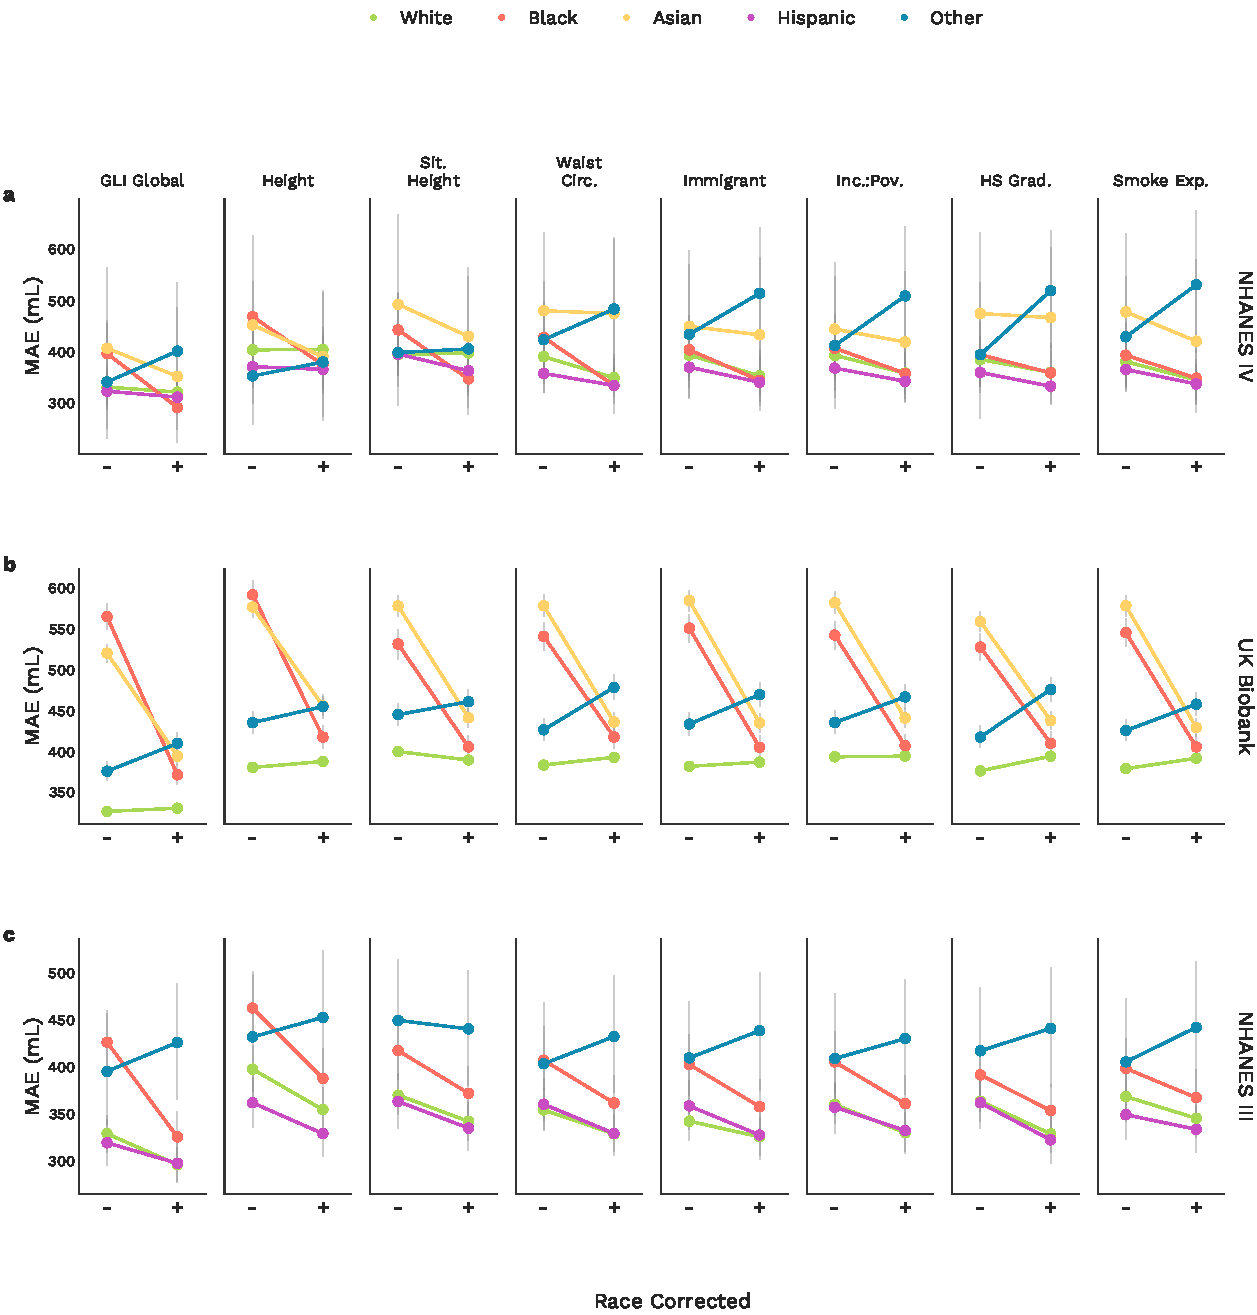
\includegraphics[width=\textwidth,height=0.78\textheight,keepaspectratio]{figures/train_fev1_nh4.pdf}
\caption{\textbf{Performance of GLI-Global and ARC\textsubscript{PFT} Models on Reference FEV$_1$ Prediction.} Models were trained on NHANES IV ($n$ = 1,249) with age, sex, and height as baseline predictors; sitting height, waist circumference, immigration status, and smoke exposure were incrementally added. MAE is shown for each race group with and without race adjustment. \textbf{(A)}~In-distribution evaluation on the NHANES IV held-out test set ($n$ = 536). \textbf{(B)}~Out-of-distribution evaluation on UK Biobank ($n$ = 144,198). \textbf{(C)}~Out-of-distribution evaluation on NHANES III ($n$ = 1,569).}
\label{fig:train_fev1_nh4}
\vspace{2pt}
\end{figure}
\clearpage

\section*{Tables}
\setcounter{table}{0}
\renewcommand{\tablename}{Supplementary Table}
\renewcommand{\thetable}{\arabic{table}}

\begin{table}[ht]
\centering
\caption{Study Population Demographics by Race — UK Biobank and Expanded NHANES Cohorts. Values are mean (SD) or $n$ (\%). Race and ethnicity were self-reported. UK Biobank does not include Hispanic participants; NHANES White, Black, and Asian categories represent non-Hispanic individuals.}
\footnotesize
\label{tab:demographics}
\adjustbox{max width=\textwidth}{%
\small
\begin{tabular}{lrrrrrrrrrrrrr}
\toprule
 & \multicolumn{4}{c}{UK Biobank} & \multicolumn{4}{c}{NHANES III} & \multicolumn{5}{c}{NHANES IV} \\
\cmidrule(lr){2-5}
\cmidrule(lr){6-9}
\cmidrule(lr){10-14}
 & White & Black & Asian & Other & White & Black & Other & Hispanic & White & Black & Asian & Other & Hispanic \\
\midrule
Sample Size & 136520 & 1963 & 3389 & 2326 & 697 & 367 & 85 & 420 & 633 & 372 & 88 & 63 & 629 \\
Age (years) & 56.9 (7.9) & 52.1 (7.8) & 53.6 (8.1) & 53.5 (8.0) & 58.7 (12.2) & 53.8 (11.7) & 53.3 (9.8) & 54.0 (11.0) & 57.1 (11.8) & 54.6 (10.3) & 53.4 (9.7) & 52.1 (10.2) & 53.9 (10.2) \\
FEV1 (mL) & 2890.5 (717.1) & 2394.0 (629.3) & 2296.2 (624.7) & 2689.4 (704.6) & 2895.0 (788.7) & 2545.0 (730.1) & 2550.2 (706.8) & 2784.6 (705.4) & 2991.8 (809.5) & 2551.1 (645.9) & 2430.0 (678.6) & 2631.0 (699.0) & 2765.5 (725.0) \\
FVC (mL) & 3717.7 (912.8) & 3016.9 (782.0) & 2905.4 (783.3) & 3417.8 (895.4) & 3670.2 (999.3) & 3136.5 (928.0) & 3150.8 (868.4) & 3446.5 (887.1) & 3832.4 (1036.2) & 3188.6 (795.5) & 3049.0 (878.7) & 3289.7 (866.1) & 3455.1 (909.6) \\
FEV1/FVC & 777.9 (38.9) & 793.7 (40.2) & 790.6 (39.5) & 787.7 (40.3) & 790.5 (53.0) & 821.0 (127.3) & 811.6 (47.2) & 810.7 (55.2) & 781.9 (47.0) & 800.9 (48.8) & 799.5 (52.0) & 800.1 (43.7) & 801.5 (44.5) \\
Height (cm) & 167.8 (9.0) & 166.5 (8.3) & 162.8 (8.9) & 165.6 (9.1) & 165.7 (9.3) & 166.7 (9.0) & 160.9 (9.0) & 160.2 (8.9) & 167.7 (10.2) & 167.4 (9.1) & 160.2 (8.6) & 162.4 (8.5) & 160.5 (9.2) \\
Sitting Height (cm) & 89.0 (4.7) & 85.7 (4.4) & 85.4 (4.8) & 87.4 (5.0) & 87.2 (4.8) & 85.5 (4.5) & 85.0 (5.1) & 85.0 (4.6) & 87.6 (4.8) & 87.1 (4.3) & 84.9 (4.2) & 85.6 (4.0) & 84.6 (4.5) \\
Waist Circ. (cm) & 88.6 (13.0) & 91.4 (12.0) & 88.3 (12.1) & 88.7 (12.9) & 93.1 (13.0) & 98.3 (13.4) & 88.4 (11.5) & 95.8 (10.5) & 101.9 (14.7) & 102.4 (15.8) & 87.6 (9.7) & 94.2 (16.0) & 99.1 (12.4) \\
Female (\%) & 60.5\% & 62.8\% & 54.8\% & 59.9\% & 67.7\% & 67.0\% & 68.2\% & 66.0\% & 58.9\% & 63.4\% & 62.5\% & 60.3\% & 63.0\% \\
Immigrant (\%) & 4.0\% & 69.5\% & 88.3\% & 50.5\% & 5.0\% & 9.8\% & 91.8\% & 43.8\% & 6.3\% & 19.4\% & 97.7\% & 74.6\% & 73.9\% \\
Education (\%) & 56.5\% & 63.5\% & 64.0\% & 66.0\% & 44.2\% & 28.3\% & 42.4\% & 13.3\% & 87.5\% & 78.0\% & 77.3\% & 77.8\% & 49.6\% \\
Smoke Exposure (\%) & 18.8\% & 12.4\% & 12.8\% & 16.9\% & 20.5\% & 36.2\% & 31.8\% & 26.0\% & 6.5\% & 8.9\% & 3.4\% & 1.6\% & 3.8\% \\
Above Poverty (\%) & 84.4\% & 78.3\% & 80.5\% & 80.8\% & 94.0\% & 79.0\% & 81.2\% & 67.6\% & 89.7\% & 85.5\% & 79.5\% & 71.4\% & 74.4\% \\
\bottomrule
\end{tabular}%
}
\end{table}
\clearpage

\begin{table}[ht]
\centering
\caption{Cumulative Race-Adjusted FVC Difference Explained in UK Biobank. Covariates were added one at a time to a baseline model (age and sex). The race coefficient (mL), percentage of the baseline race difference explained, and model MSE are reported after including each covariate and all preceding ones.}
\footnotesize
\label{tab:explain_fvc_ukb}
\vspace{4pt}
\adjustbox{max width=\textwidth}{%
\small
\begin{tabular}{lrrrrrrr}
\toprule
Variable & \multicolumn{2}{c}{Asian} & \multicolumn{2}{c}{Black} & \multicolumn{2}{c}{Other} &  \\
\cmidrule(lr){2-3}
\cmidrule(lr){4-5}
\cmidrule(lr){6-7}
 & mL & \% & mL & \% & mL & \% & MSE \\
\midrule
Baseline & -1003 & 0 & -846 & 0 & -430 & 0 & 376,000 \\
Height & -715 & 29 & -758 & 10 & -300 & 30 & 285,140 \\
Waist Circ. & -701 & 30 & -726 & 14 & -286 & 33 & 272,566 \\
Sit. Height & -685 & 32 & -682 & 19 & -278 & 35 & 271,524 \\
Immigrant & -624 & 38 & -639 & 24 & -246 & 43 & 272,338 \\
Work Air & -622 & 38 & -637 & 25 & -244 & 43 & 272,203 \\
PM10 & -619 & 38 & -633 & 25 & -242 & 44 & 272,085 \\
HS Grad. & -618 & 38 & -632 & 25 & -242 & 44 & 272,003 \\
Weight & -618 & 38 & -632 & 25 & -241 & 44 & 271,716 \\
BMI & -618 & 38 & -634 & 25 & -241 & 44 & 271,352 \\
\bottomrule
\end{tabular}%
}
\end{table}
\clearpage

\begin{table}[ht]
\centering
\caption{Cumulative Race-Adjusted FVC Difference Explained in NHANES (III and IV Combined). Covariates were added one at a time to a baseline model (age and sex). The race coefficient (mL), percentage of the baseline race difference explained, and model MSE are reported after including each covariate and all preceding ones.}
\footnotesize
\label{tab:explain_fvc_nh}
\vspace{4pt}
\adjustbox{max width=\textwidth}{%
\small
\begin{tabular}{lrrrrrrrrr}
\toprule
Variable & \multicolumn{2}{c}{Asian} & \multicolumn{2}{c}{Black} & \multicolumn{2}{c}{Hispanic} & \multicolumn{2}{c}{Other} &  \\
\cmidrule(lr){2-3}
\cmidrule(lr){4-5}
\cmidrule(lr){6-7}
\cmidrule(lr){8-9}
 & mL & \% & mL & \% & mL & \% & mL & \% & MSE \\
\midrule
Baseline & -860 & 0 & -685 & 0 & -418 & 0 & -688 & 0 & 349,363 \\
Height & -501 & 42 & -680 & 1 & -87 & 79 & -401 & 42 & 250,491 \\
Waist Circ. & -551 & 36 & -664 & 3 & -70 & 83 & -426 & 38 & 241,779 \\
Sit. Height & -551 & 36 & -598 & 13 & -60 & 86 & -429 & 38 & 235,321 \\
Arm Length & -555 & 35 & -614 & 10 & -56 & 87 & -425 & 38 & 237,970 \\
Immigrant & -496 & 42 & -610 & 11 & -23 & 95 & -367 & 47 & 237,929 \\
Eng. Lang. & -497 & 42 & -606 & 12 & -49 & 88 & -373 & 46 & 237,411 \\
BMI & -484 & 44 & -617 & 10 & -50 & 88 & -362 & 47 & 235,486 \\
Arm Circ. & -479 & 44 & -609 & 11 & -51 & 88 & -359 & 48 & 234,114 \\
Veteran & -493 & 43 & -607 & 11 & -48 & 88 & -374 & 46 & 235,921 \\
\bottomrule
\end{tabular}%
}
\end{table}
\clearpage

\begin{table}[ht]
\centering
\caption{Cumulative Race-Adjusted FVC Difference Explained in NHANES III. Covariates were added one at a time to a baseline model (age and sex). The race coefficient (mL), percentage of the baseline race difference explained, and model MSE are reported after including each covariate and all preceding ones.}
\footnotesize
\label{tab:explain_fvc_nh3}
\vspace{4pt}
\adjustbox{max width=\textwidth}{%
\small
\begin{tabular}{lrrrrrrr}
\toprule
Variable & \multicolumn{2}{c}{Black} & \multicolumn{2}{c}{Hispanic} & \multicolumn{2}{c}{Other} &  \\
\cmidrule(lr){2-3}
\cmidrule(lr){4-5}
\cmidrule(lr){6-7}
 & mL & \% & mL & \% & mL & \% & MSE \\
\midrule
Baseline & -695 & 0 & -392 & 0 & -682 & 0 & 354,363 \\
Height & -707 & -2 & -87 & 78 & -416 & 39 & 263,786 \\
Sit. Height & -598 & 14 & -76 & 81 & -403 & 41 & 254,658 \\
Waist Circ. & -559 & 19 & -59 & 85 & -403 & 41 & 249,015 \\
Arm Length & -566 & 18 & -42 & 89 & -408 & 40 & 249,699 \\
Inc.:Pov. & -559 & 19 & -28 & 93 & -395 & 42 & 249,277 \\
Veteran & -558 & 20 & -27 & 93 & -387 & 43 & 248,911 \\
Work Mask & -557 & 20 & -26 & 93 & -385 & 44 & 248,677 \\
Arm Circ. & -548 & 21 & -37 & 91 & -374 & 45 & 244,471 \\
BMI & -562 & 19 & -36 & 91 & -376 & 45 & 244,806 \\
\bottomrule
\end{tabular}%
}
\end{table}
\clearpage

\begin{table}[ht]
\centering
\caption{Cumulative Race-Adjusted FVC Difference Explained in NHANES IV. Covariates were added one at a time to a baseline model (age and sex). The race coefficient (mL), percentage of the baseline race difference explained, and model MSE are reported after including each covariate and all preceding ones.}
\footnotesize
\label{tab:explain_fvc_nh4}
\vspace{4pt}
\adjustbox{max width=\textwidth}{%
\small
\begin{tabular}{lrrrrrrrrr}
\toprule
Variable & \multicolumn{2}{c}{Asian} & \multicolumn{2}{c}{Black} & \multicolumn{2}{c}{Hispanic} & \multicolumn{2}{c}{Other} &  \\
\cmidrule(lr){2-3}
\cmidrule(lr){4-5}
\cmidrule(lr){6-7}
\cmidrule(lr){8-9}
 & mL & \% & mL & \% & mL & \% & mL & \% & MSE \\
\midrule
Baseline & -868 & 0 & -673 & 0 & -439 & 0 & -698 & 0 & 341,917 \\
Height & -487 & 44 & -652 & 3 & -84 & 81 & -388 & 44 & 236,977 \\
Waist Circ. & -578 & 33 & -655 & 3 & -79 & 82 & -437 & 37 & 226,152 \\
BMI & -559 & 36 & -663 & 1 & -72 & 83 & -424 & 39 & 224,861 \\
Arm Circ. & -556 & 36 & -655 & 3 & -68 & 84 & -424 & 39 & 224,132 \\
Mineral Dust & -547 & 37 & -653 & 3 & -64 & 85 & -420 & 40 & 222,587 \\
Immigrant & -496 & 43 & -641 & 5 & -20 & 95 & -380 & 45 & 222,898 \\
Eng. Lang. & -490 & 44 & -634 & 6 & -47 & 89 & -375 & 46 & 221,911 \\
Sit. Height & -497 & 43 & -617 & 8 & -51 & 88 & -368 & 47 & 217,246 \\
Arm Length & -504 & 42 & -633 & 6 & -47 & 89 & -383 & 45 & 219,379 \\
\bottomrule
\end{tabular}%
}
\end{table}
\clearpage

\begin{table}[ht]
\centering
\caption{Cumulative Race-Adjusted FEV$_1$ Difference Explained in UK Biobank. Covariates were added one at a time to a baseline model (age and sex). The race coefficient (mL), percentage of the baseline race difference explained, and model MSE are reported after including each covariate and all preceding ones.}
\footnotesize
\label{tab:explain_fev1_ukb}
\vspace{4pt}
\adjustbox{max width=\textwidth}{%
\small
\begin{tabular}{lrrrrrrr}
\toprule
Variable & \multicolumn{2}{c}{Asian} & \multicolumn{2}{c}{Black} & \multicolumn{2}{c}{Other} &  \\
\cmidrule(lr){2-3}
\cmidrule(lr){4-5}
\cmidrule(lr){6-7}
 & mL & \% & mL & \% & mL & \% & MSE \\
\midrule
Baseline & -756 & 0 & -629 & 0 & -316 & 0 & 225,988 \\
Height & -549 & 27 & -566 & 10 & -223 & 29 & 179,531 \\
Waist Circ. & -540 & 29 & -548 & 13 & -214 & 32 & 174,397 \\
Sit. Height & -528 & 30 & -515 & 18 & -208 & 34 & 174,062 \\
Work Air & -520 & 31 & -511 & 19 & -204 & 35 & 174,412 \\
HS Grad. & -522 & 31 & -513 & 19 & -206 & 35 & 174,323 \\
Immigrant & -485 & 36 & -484 & 23 & -186 & 41 & 174,231 \\
PM10 & -483 & 36 & -481 & 24 & -184 & 42 & 174,167 \\
BMI & -481 & 36 & -487 & 23 & -184 & 42 & 173,789 \\
Weight & -479 & 37 & -487 & 23 & -183 & 42 & 173,908 \\
\bottomrule
\end{tabular}%
}
\end{table}
\clearpage

\begin{table}[ht]
\centering
\caption{Cumulative Race-Adjusted FEV$_1$ Difference Explained in NHANES (III and IV Combined). Covariates were added one at a time to a baseline model (age and sex). The race coefficient (mL), percentage of the baseline race difference explained, and model MSE are reported after including each covariate and all preceding ones.}
\footnotesize
\label{tab:explain_fev1_nh}
\vspace{4pt}
\adjustbox{max width=\textwidth}{%
\small
\begin{tabular}{lrrrrrrrrr}
\toprule
Variable & \multicolumn{2}{c}{Asian} & \multicolumn{2}{c}{Black} & \multicolumn{2}{c}{Hispanic} & \multicolumn{2}{c}{Other} &  \\
\cmidrule(lr){2-3}
\cmidrule(lr){4-5}
\cmidrule(lr){6-7}
\cmidrule(lr){8-9}
 & mL & \% & mL & \% & mL & \% & mL & \% & MSE \\
\midrule
Baseline & -659 & 0 & -489 & 0 & -283 & 0 & -497 & 0 & 202,872 \\
Height & -403 & 39 & -485 & 1 & -47 & 83 & -292 & 41 & 152,480 \\
Waist Circ. & -435 & 34 & -474 & 3 & -35 & 88 & -308 & 38 & 148,880 \\
Sit. Height & -437 & 34 & -424 & 13 & -28 & 90 & -310 & 37 & 144,784 \\
Immigrant & -377 & 43 & -425 & 13 & 10 & 104 & -255 & 49 & 146,580 \\
BMI & -363 & 45 & -438 & 11 & 8 & 103 & -244 & 51 & 145,186 \\
Arm Circ. & -361 & 45 & -431 & 12 & 10 & 104 & -244 & 51 & 144,752 \\
Arm Length & -373 & 43 & -430 & 12 & 15 & 105 & -255 & 49 & 145,257 \\
Eng. Lang. & -371 & 44 & -429 & 12 & -1 & 100 & -252 & 49 & 145,310 \\
Veteran & -372 & 44 & -429 & 12 & -2 & 99 & -253 & 49 & 145,120 \\
\bottomrule
\end{tabular}%
}
\end{table}
\clearpage

\begin{table}[ht]
\centering
\caption{Cumulative Race-Adjusted FEV$_1$ Difference Explained in NHANES III. Covariates were added one at a time to a baseline model (age and sex). The race coefficient (mL), percentage of the baseline race difference explained, and model MSE are reported after including each covariate and all preceding ones.}
\footnotesize
\label{tab:explain_fev1_nh3}
\vspace{4pt}
\adjustbox{max width=\textwidth}{%
\small
\begin{tabular}{lrrrrrrr}
\toprule
Variable & \multicolumn{2}{c}{Black} & \multicolumn{2}{c}{Hispanic} & \multicolumn{2}{c}{Other} &  \\
\cmidrule(lr){2-3}
\cmidrule(lr){4-5}
\cmidrule(lr){6-7}
 & mL & \% & mL & \% & mL & \% & MSE \\
\midrule
Baseline & -500 & 0 & -264 & 0 & -494 & 0 & 200,706 \\
Height & -509 & -2 & -43 & 84 & -300 & 39 & 152,278 \\
Sit. Height & -428 & 14 & -33 & 87 & -290 & 41 & 147,631 \\
Waist Circ. & -399 & 20 & -20 & 93 & -291 & 41 & 144,979 \\
Arm Length & -404 & 19 & -9 & 96 & -295 & 40 & 144,997 \\
Immigrant & -403 & 19 & 9 & 103 & -248 & 50 & 144,825 \\
Inc.:Pov. & -399 & 20 & 16 & 106 & -247 & 50 & 144,592 \\
Work Mask & -398 & 20 & 17 & 106 & -245 & 50 & 144,427 \\
Health Insurance & -396 & 21 & 14 & 105 & -245 & 50 & 144,312 \\
HS Grad. & -392 & 22 & 20 & 108 & -246 & 50 & 144,183 \\
\bottomrule
\end{tabular}%
}
\end{table}
\clearpage

\begin{table}[ht]
\centering
\caption{Cumulative Race-Adjusted FEV$_1$ Difference Explained in NHANES IV. Covariates were added one at a time to a baseline model (age and sex). The race coefficient (mL), percentage of the baseline race difference explained, and model MSE are reported after including each covariate and all preceding ones.}
\footnotesize
\label{tab:explain_fev1_nh4}
\vspace{4pt}
\adjustbox{max width=\textwidth}{%
\small
\begin{tabular}{lrrrrrrrrr}
\toprule
Variable & \multicolumn{2}{c}{Asian} & \multicolumn{2}{c}{Black} & \multicolumn{2}{c}{Hispanic} & \multicolumn{2}{c}{Other} &  \\
\cmidrule(lr){2-3}
\cmidrule(lr){4-5}
\cmidrule(lr){6-7}
\cmidrule(lr){8-9}
 & mL & \% & mL & \% & mL & \% & mL & \% & MSE \\
\midrule
Baseline & -646 & 0 & -475 & 0 & -291 & 0 & -505 & 0 & 202,115 \\
Height & -379 & 41 & -460 & 3 & -43 & 85 & -288 & 43 & 150,224 \\
Waist Circ. & -430 & 33 & -463 & 2 & -39 & 87 & -316 & 38 & 146,988 \\
Immigrant & -367 & 43 & -453 & 5 & 12 & 104 & -269 & 47 & 146,421 \\
BMI & -348 & 46 & -461 & 3 & 13 & 105 & -255 & 50 & 145,096 \\
Arm Circ. & -349 & 46 & -455 & 4 & 16 & 106 & -259 & 49 & 144,890 \\
Sit. Height & -366 & 43 & -439 & 8 & 13 & 104 & -259 & 49 & 142,198 \\
Eng. Lang. & -362 & 44 & -444 & 7 & 0 & 100 & -263 & 48 & 144,477 \\
Mineral Dust & -357 & 45 & -444 & 7 & -0 & 100 & -261 & 48 & 143,892 \\
Military Health & -359 & 45 & -442 & 7 & 1 & 100 & -261 & 48 & 143,973 \\
\bottomrule
\end{tabular}%
}
\end{table}
\clearpage

\begin{table}[ht]
\centering
\caption{Category-Level Race-Adjusted FEV$_1$ and FVC Difference Explained in UK Biobank. Each covariate category (anthropometrics, sociodemographics, exposures) was tested independently from a baseline model of age and sex. $P$ is the maximum $p$-value across both outcomes for that race, adjusted for age and sex.}
\footnotesize
\label{tab:explain_ukb_reset}
\vspace{4pt}
\adjustbox{max width=\textwidth}{%
\small
\begin{tabular}{lrrrrrrrrrrrrrrr}
\toprule
 & \multicolumn{5}{c}{Black} & \multicolumn{5}{c}{Asian} & \multicolumn{5}{c}{Other} \\
\cmidrule(lr){2-6}
\cmidrule(lr){7-11}
\cmidrule(lr){12-16}
 & \multicolumn{2}{c}{FEV$_1$} & \multicolumn{2}{c}{FVC} &  & \multicolumn{2}{c}{FEV$_1$} & \multicolumn{2}{c}{FVC} &  & \multicolumn{2}{c}{FEV$_1$} & \multicolumn{2}{c}{FVC} &  \\
\cmidrule(lr){2-3}
\cmidrule(lr){4-5}
\cmidrule(lr){7-8}
\cmidrule(lr){9-10}
\cmidrule(lr){12-13}
\cmidrule(lr){14-15}
Variable & Coef. & \% & Coef. & \% & $P$ & Coef. & \% & Coef. & \% & $P$ & Coef. & \% & Coef. & \% & $P$ \\
\midrule
Baseline & -629 & 0 & -846 & 0 & $<$0.001 & -756 & 0 & -1003 & 0 & $<$0.001 & -316 & 0 & -430 & 0 & $<$0.001 \\
Anthropometrics & -518 & 18 & -679 & 20 & $<$0.001 & -518 & 32 & -675 & 33 & $<$0.001 & -204 & 35 & -272 & 37 & $<$0.001 \\
Sociodemographics & -594 & 6 & -796 & 6 & $<$0.001 & -715 & 5 & -944 & 6 & $<$0.001 & -295 & 7 & -399 & 7 & $<$0.001 \\
Exposures & -609 & 3 & -821 & 3 & $<$0.001 & -742 & 2 & -985 & 2 & $<$0.001 & -303 & 4 & -414 & 4 & $<$0.001 \\
\bottomrule
\end{tabular}%
}
\end{table}
\clearpage

\begin{table}[ht]
\centering
\caption{Category-Level Race-Adjusted FEV$_1$ and FVC Difference Explained in NHANES (III and IV Combined). Each covariate category (anthropometrics, sociodemographics, exposures) was tested independently from a baseline model of age and sex. $P$ is the maximum $p$-value across both outcomes for that race, adjusted for age and sex.}
\footnotesize
\label{tab:explain_nh_reset}
\vspace{4pt}
\adjustbox{max width=\textwidth}{%
\small
\begin{tabular}{lrrrrrrrrrrrrrrrrrrrr}
\toprule
 & \multicolumn{5}{c}{Black} & \multicolumn{5}{c}{Asian} & \multicolumn{5}{c}{Hispanic} & \multicolumn{5}{c}{Other} \\
\cmidrule(lr){2-6}
\cmidrule(lr){7-11}
\cmidrule(lr){12-16}
\cmidrule(lr){17-21}
 & \multicolumn{2}{c}{FEV$_1$} & \multicolumn{2}{c}{FVC} &  & \multicolumn{2}{c}{FEV$_1$} & \multicolumn{2}{c}{FVC} &  & \multicolumn{2}{c}{FEV$_1$} & \multicolumn{2}{c}{FVC} &  & \multicolumn{2}{c}{FEV$_1$} & \multicolumn{2}{c}{FVC} &  \\
\cmidrule(lr){2-3}
\cmidrule(lr){4-5}
\cmidrule(lr){7-8}
\cmidrule(lr){9-10}
\cmidrule(lr){12-13}
\cmidrule(lr){14-15}
\cmidrule(lr){17-18}
\cmidrule(lr){19-20}
Variable & Coef. & \% & Coef. & \% & $P$ & Coef. & \% & Coef. & \% & $P$ & Coef. & \% & Coef. & \% & $P$ & Coef. & \% & Coef. & \% & $P$ \\
\midrule
Baseline & -489 & 0 & -685 & 0 & $<$0.001 & -659 & 0 & -860 & 0 & $<$0.001 & -283 & 0 & -418 & 0 & $<$0.001 & -497 & 0 & -688 & 0 & $<$0.001 \\
Anthropometrics & -440 & 10 & -619 & 10 & $<$0.001 & -423 & 36 & -536 & 38 & $<$0.001 & -25 & 91 & -56 & 87 & 0.159 & -293 & 41 & -404 & 41 & $<$0.001 \\
Sociodemographics & -444 & 9 & -626 & 9 & $<$0.001 & -530 & 19 & -716 & 17 & $<$0.001 & -169 & 40 & -286 & 32 & $<$0.001 & -367 & 26 & -537 & 22 & $<$0.001 \\
Exposures & -487 & 0 & -682 & 0 & $<$0.001 & -661 & -0 & -865 & -1 & $<$0.001 & -283 & -0 & -419 & -0 & $<$0.001 & -496 & 0 & -687 & 0 & $<$0.001 \\
\bottomrule
\end{tabular}%
}
\end{table}
\clearpage

\begin{table}[ht]
\centering
\caption{Category-Level Race-Adjusted FEV$_1$ and FVC Difference Explained in NHANES III. Each covariate category (anthropometrics, sociodemographics, exposures) was tested independently from a baseline model of age and sex. $P$ is the maximum $p$-value across both outcomes for that race, adjusted for age and sex.}
\footnotesize
\label{tab:explain_nh3_reset}
\vspace{4pt}
\adjustbox{max width=\textwidth}{%
\small
\begin{tabular}{lrrrrrrrrrrrrrrr}
\toprule
 & \multicolumn{5}{c}{Black} & \multicolumn{5}{c}{Hispanic} & \multicolumn{5}{c}{Other} \\
\cmidrule(lr){2-6}
\cmidrule(lr){7-11}
\cmidrule(lr){12-16}
 & \multicolumn{2}{c}{FEV$_1$} & \multicolumn{2}{c}{FVC} &  & \multicolumn{2}{c}{FEV$_1$} & \multicolumn{2}{c}{FVC} &  & \multicolumn{2}{c}{FEV$_1$} & \multicolumn{2}{c}{FVC} &  \\
\cmidrule(lr){2-3}
\cmidrule(lr){4-5}
\cmidrule(lr){7-8}
\cmidrule(lr){9-10}
\cmidrule(lr){12-13}
\cmidrule(lr){14-15}
Variable & Coef. & \% & Coef. & \% & $P$ & Coef. & \% & Coef. & \% & $P$ & Coef. & \% & Coef. & \% & $P$ \\
\midrule
Baseline & -500 & 0 & -695 & 0 & $<$0.001 & -264 & 0 & -392 & 0 & $<$0.001 & -494 & 0 & -682 & 0 & $<$0.001 \\
Anthropometrics & -408 & 18 & -567 & 18 & $<$0.001 & -14 & 95 & -50 & 87 & 0.585 & -282 & 43 & -388 & 43 & $<$0.001 \\
Sociodemographics & -438 & 12 & -611 & 12 & $<$0.001 & -149 & 44 & -251 & 36 & $<$0.001 & -360 & 27 & -518 & 24 & $<$0.001 \\
Exposures & -495 & 1 & -689 & 1 & $<$0.001 & -263 & 0 & -391 & 0 & $<$0.001 & -490 & 1 & -678 & 1 & $<$0.001 \\
\bottomrule
\end{tabular}%
}
\end{table}
\clearpage

\begin{table}[ht]
\centering
\caption{Category-Level Race-Adjusted FEV$_1$ and FVC Difference Explained in NHANES IV. Each covariate category (anthropometrics, sociodemographics, exposures) was tested independently from a baseline model of age and sex. $P$ is the maximum $p$-value across both outcomes for that race, adjusted for age and sex.}
\footnotesize
\label{tab:explain_nh4_reset}
\vspace{4pt}
\adjustbox{max width=\textwidth}{%
\small
\begin{tabular}{lrrrrrrrrrrrrrrrrrrrr}
\toprule
 & \multicolumn{5}{c}{Black} & \multicolumn{5}{c}{Asian} & \multicolumn{5}{c}{Hispanic} & \multicolumn{5}{c}{Other} \\
\cmidrule(lr){2-6}
\cmidrule(lr){7-11}
\cmidrule(lr){12-16}
\cmidrule(lr){17-21}
 & \multicolumn{2}{c}{FEV$_1$} & \multicolumn{2}{c}{FVC} &  & \multicolumn{2}{c}{FEV$_1$} & \multicolumn{2}{c}{FVC} &  & \multicolumn{2}{c}{FEV$_1$} & \multicolumn{2}{c}{FVC} &  & \multicolumn{2}{c}{FEV$_1$} & \multicolumn{2}{c}{FVC} &  \\
\cmidrule(lr){2-3}
\cmidrule(lr){4-5}
\cmidrule(lr){7-8}
\cmidrule(lr){9-10}
\cmidrule(lr){12-13}
\cmidrule(lr){14-15}
\cmidrule(lr){17-18}
\cmidrule(lr){19-20}
Variable & Coef. & \% & Coef. & \% & $P$ & Coef. & \% & Coef. & \% & $P$ & Coef. & \% & Coef. & \% & $P$ & Coef. & \% & Coef. & \% & $P$ \\
\midrule
Baseline & -475 & 0 & -673 & 0 & $<$0.001 & -646 & 0 & -868 & 0 & $<$0.001 & -291 & 0 & -439 & 0 & $<$0.001 & -505 & 0 & -698 & 0 & $<$0.001 \\
Anthropometrics & -461 & 3 & -654 & 3 & $<$0.001 & -419 & 35 & -562 & 35 & $<$0.001 & -32 & 89 & -68 & 85 & 0.192 & -305 & 40 & -421 & 40 & $<$0.001 \\
Sociodemographics & -442 & 7 & -630 & 6 & $<$0.001 & -528 & 18 & -730 & 16 & $<$0.001 & -177 & 39 & -311 & 29 & $<$0.001 & -401 & 21 & -571 & 18 & $<$0.001 \\
Exposures & -476 & -0 & -673 & -0 & $<$0.001 & -642 & 1 & -861 & 1 & $<$0.001 & -290 & 0 & -439 & -0 & $<$0.001 & -504 & 0 & -697 & 0 & $<$0.001 \\
\bottomrule
\end{tabular}%
}
\end{table}
\clearpage

\end{document}
